\documentclass[11pt,twoside]{scrreprt}

\renewcommand{\textfraction}{0.001}
\renewcommand{\topfraction}{0.999}   
\renewcommand{\bottomfraction}{0.999}

\usepackage{graphicx}
\usepackage{amsmath}
\usepackage{mathtools}
\usepackage{amssymb}
\usepackage[bibencoding=utf8, backend=biber, style=numeric-comp, sorting=none, minbibnames=1, maxnames=5]{biblatex}
\addbibresource{bibliography.bib}
\usepackage{a4,color}
\usepackage{tikz}
\usepackage{pgfplots}
\pgfplotsset{compat=1.10}
\usepackage{calc}

\usepackage{booktabs}
\usepackage{caption}
\usepackage{longtable}
% \usepackage{subcaption}
\usepackage{float}
\usepackage{url}
\usepackage{listings}
\usepackage{hyperref}
\usepackage{subfig}
\usepackage[top=3.5cm, bottom=3.7cm, left=3cm, right=3cm]{geometry}

\usepackage[T1]{fontenc}
\usepackage[utf8]{inputenc}

\usepackage{mathpazo}

\definecolor{red}{rgb}{1,0,0}
\definecolor{green}{rgb}{0,1,0}
\definecolor{blue}{rgb}{0,0,1}
\definecolor{darkblue}{rgb}{0,0,0.8}

\definecolor{yellow}{rgb}{1,1,0}
\definecolor{lightblue}{rgb}{0,1,1}
\definecolor{magenta}{rgb}{1,0,1}
\definecolor{lightgrey}{rgb}{0.5,0.5,0.5}
\definecolor{grey}{rgb}{0.35,0.35,0.35}
\definecolor{darkgrey}{rgb}{0.2,0.2,0.2}
\definecolor{ockerrot}{rgb}{0.859,0.375,0.152}

% Default fixed font does not support bold face
\DeclareFixedFont{\ttb}{T1}{txtt}{bx}{n}{12} % for bold
\DeclareFixedFont{\ttm}{T1}{txtt}{m}{n}{12}  % for normal

% Custom colors
\usepackage{color}
\definecolor{deepblue}{rgb}{0,0,0.5}
\definecolor{deepred}{rgb}{0.6,0,0}
\definecolor{deepgreen}{rgb}{0,0.5,0}

\usepackage{listings}

% Python style for highlighting
\lstset{
language=Python,
basicstyle=\ttm,
otherkeywords={self, for},             % Add keywords here
keywordstyle=\ttb\color{deepblue},
emph={MyClass,__init__, np},          % Custom highlighting
emphstyle=\ttb\color{deepred},    % Custom highlighting style
stringstyle=\color{deepgreen},
frame=tb,                         % Any extra options here
showstringspaces=false            % 
}


\captionsetup{margin=0pt,font=small,labelfont=sc,labelformat=simple,format=plain,indention=3mm,
 labelsep=endash,textfont=sf,font=sf,singlelinecheck=on,figurename=Fig.,tablename=Tab.}


\fontfamily{ppl}\selectfont

\newcommand*{\bfrac}[2]{\genfrac{\big (}{\big )}{0pt}{}{#1}{#2}}

\setlength{\parskip}{1.5ex plus 0.5ex minus 0.2ex}
\setlength{\parindent}{0pt}

% \linespread{1.5}\selectfont

\begin{document}


\begin{titlepage}
  \includegraphics[width=0.4\textwidth]{pics/UZH_Logo_e_EPS/uzh_logo_e_pos.pdf}
  \vspace{1cm}

  \Huge\centering New Approach to the Circle Hough Transform for the LHC\textit{b} for Detecting
        Cherenkov Rings in the RICH detector

  \noindent\makebox[\textwidth]{\rule{\textwidth}{0.4pt}}

\vspace{1cm}

{\centering
  \Large Master thesis\\
  of\\
  Philipp Gloor
  \vspace{1.5cm}

  \Large Mathematisch-naturwissenschaftliche Fakultät\\
  der\\
  Universität Zürich
  \vspace{2cm}

  \Large Prof. Dr. U. Straumann\\
  Prof. Dr. P. Saha\\
  Dr. O. Steinkamp\\
\vspace*{\fill}
\Large Zürich 2016


  }
\end{titlepage}
\chapter*{Abstract}
\addcontentsline{toc}{chapter}{Abstract}
This thesis explores possible algorithms for the detection of circles of Cherenkov photons which are produced by particles 
travelling through a RICH detectors in the LHC\textit{b} experiment. These circles can be detected with the help of a Hough 
transform. There is a short introduction to the linear Hough transform (which detects straight lines) to give a rough idea about 
what the Hough transform can do. Then there is a brief look at the circle Hough transform (which detects circles). This part is 
split in 3 sections, discussing 1D, 2D and 3D Hough transforms. The 1D Hough transform can be used when the center is given and the radius 
needs to be found. The 2D Hough transform looks for the position of circle centers ($(x,y)$ coordinate) for a given radius. 
The 3D Hough transform is used when neither center nor radius are known. This is the case for the data from LHC\textit{b} 
where there are data points (photons from several circles and noise hits) and the algorithm has to find all the circles.

Apart from the standard Hough transform with a 3D accumulator space this thesis develops a new approach for a Hough transform. 
This approach works on the basis that each circle is defined by 3 points. Given 3 points one can calculate the circumcenter 
(so the center of the circle we are intersted in) and the radius of the circumcircle.

\tableofcontents
\listoftables
\listoffigures	

\chapter{Introduction}
\section{LHC - Large Hadron Collider} % (fold)
\label{sec:lhc_large_hadron_collider}
\begin{figure}[htb]
  \centering
  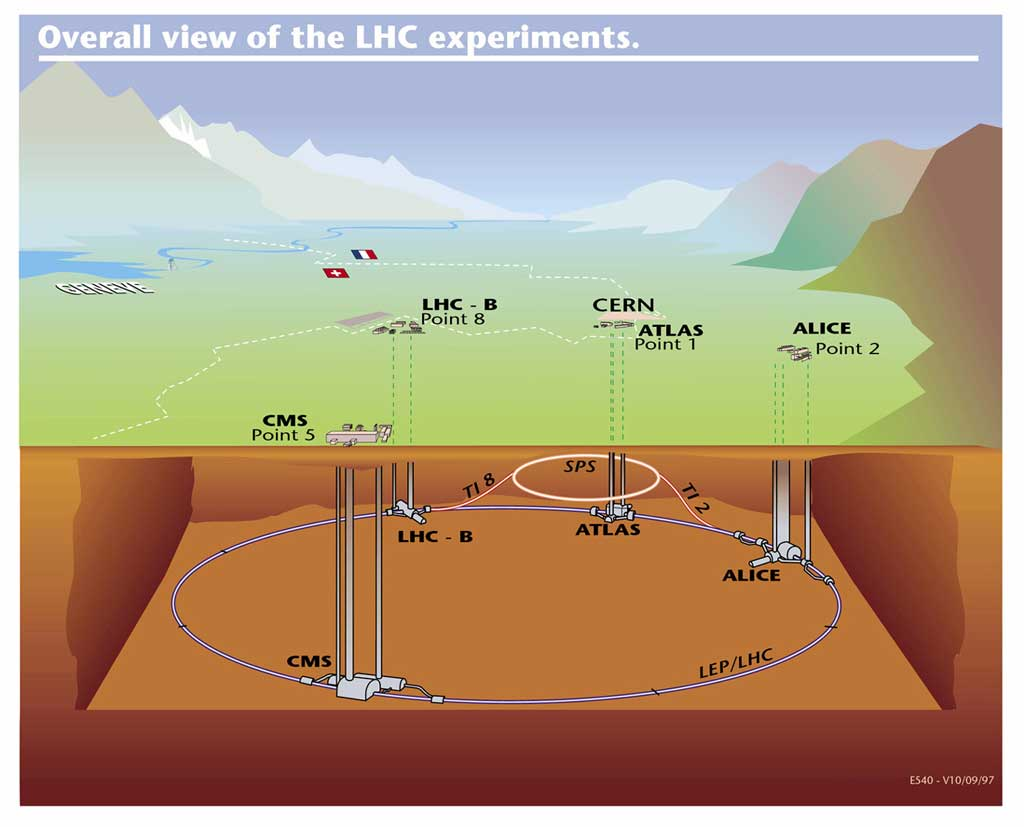
\includegraphics[width=0.6\textwidth]{pics/lhc}
  \caption{The LHC ring with its 4 experiments: ATLAS, CMS, ALICE and LHC\textit{b}}
  \label{fig:lhc}
\end{figure}

The Large Hadron Collider (LHC) is the largest and highest-energy particle accelerator in the world colliding protons on protons
at beam energies of up to $16.5$\,TeV and lead ions at beam energies up to $5.5$\,GeV/nucleon. It was built by the European 
Organisation for Nuclear Research from 1998 to 2008. It aims to test the predictions of different theories in high-energy particle 
physics, in particular for the search of the Higgs boson (which has been confirmed last year) and signs for new physics beyond 
the Standard Model of particle physics. The LHC lies in a tunnel 27\,km in circumference and up to 100\,m below the surface of the 
French-Swiss border near Geneva. The LHC was built in collaboration with over 10000 scientists and engineers from over 100 countries. 
The accelerator has been running with a center of mass energy $\sqrt{s} = 13$ TeV since 20 May 2015.

The LHC consists of 4 large experiments \parencite{Aad2008,Aamodt2008,AlvesJr2008,Collaboration2008}:

\paragraph{ATLAS/CMS}
  \begin{itemize}
    \item The two multi-purpose experiments at the LHC probing $p-p$ and heavy ions for direct searches of new particles.
  \end{itemize}
\paragraph{ALICE}
  \begin{itemize}
    \item ALICE (A Large Ion Collider Experiment) is a general-purpose, heavy ion detector at the CERN LHC
    which focuses on QCD, the strong interaction sector of the Standard Model e.g. for evidence for quark-gluon
    plasma.
  \end{itemize}
\paragraph{LHC\textit{b}}
  \begin{itemize}
    \item LHC\textit{b} is testing the Standard Model by confronting predictions with its precise measurements in CP
    violation and rare decays of particles containing $b$ and $c$ quarks.
  \end{itemize}



% section lhc_large_hadron_collider (end)

\section{LHC\textit{b}}

\begin{figure}[tb]
  \centering
  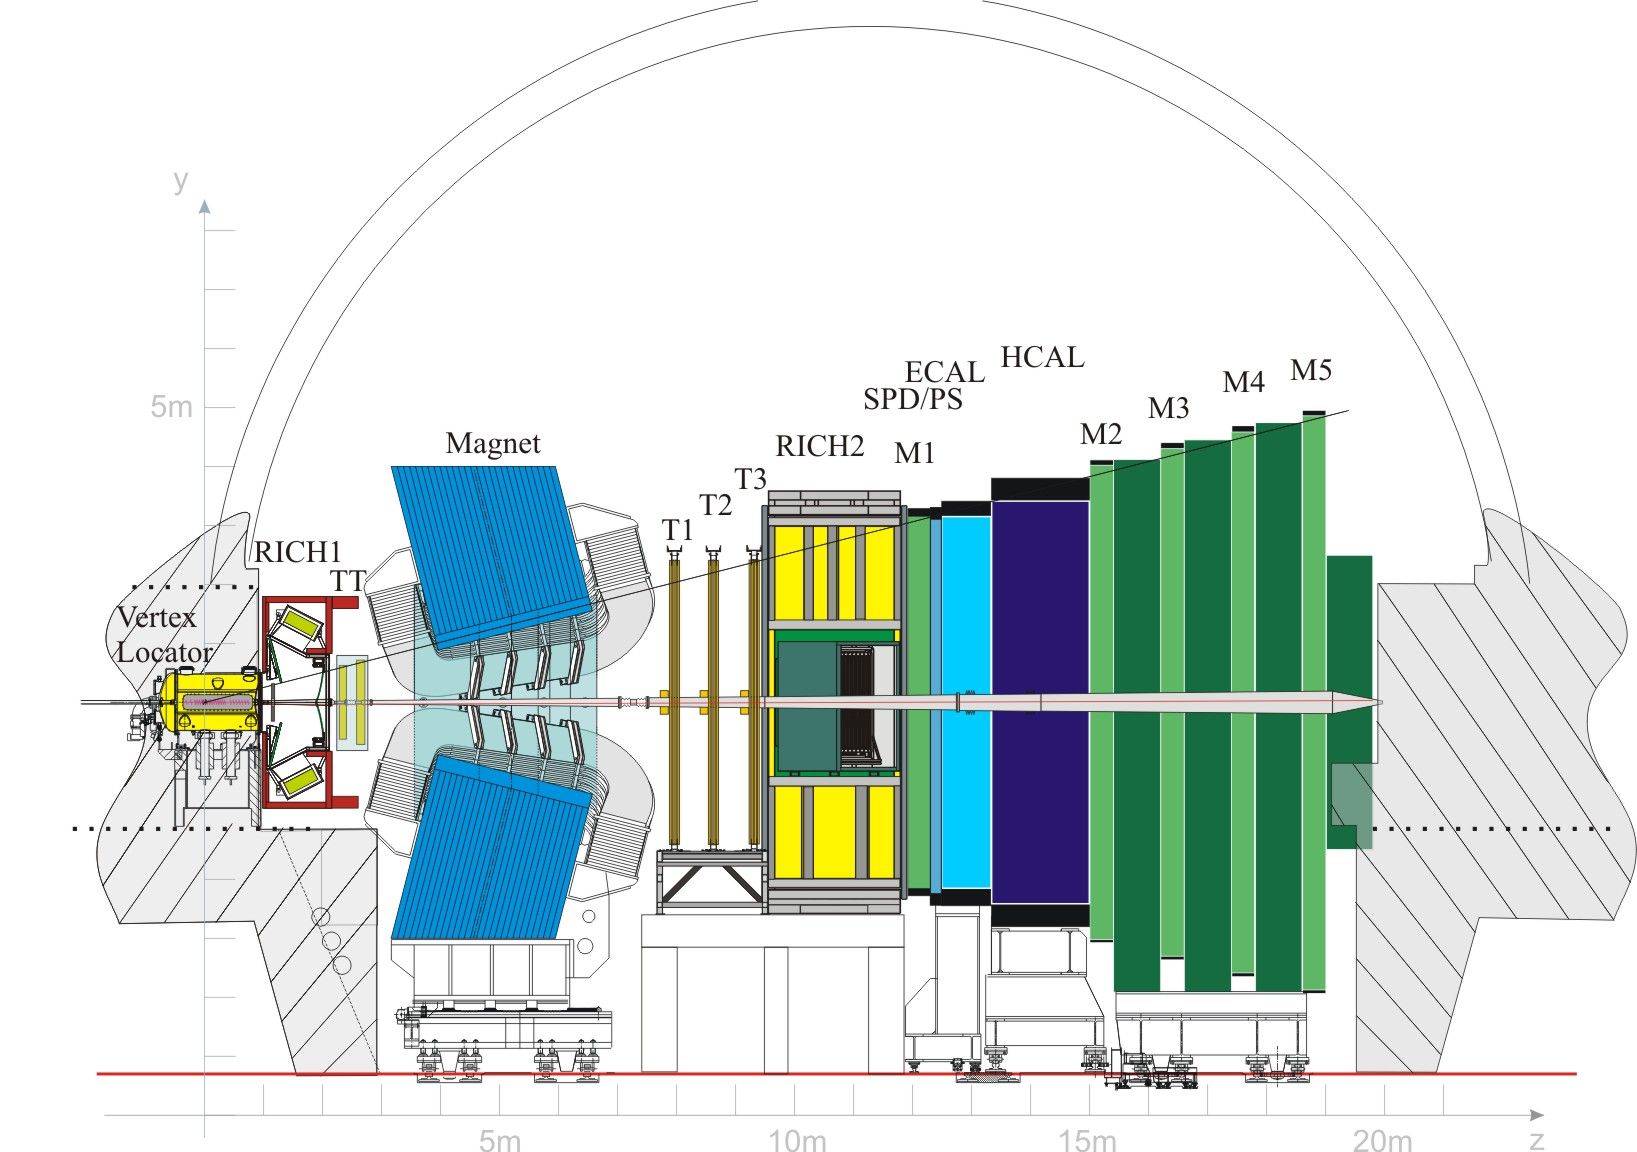
\includegraphics[width=\textwidth]{pics/lhcb_detector}
  \caption{LHC\textit{b} Detector: The beams collide inside the Vertex Locator. The RICH1 is positioned before the tracking station (TT) and
  the magnet. RICH2 is set up after the magnet and the silicon trackers (T1-T3) and before the muon and calorimeter (M1-M5)}
  \label{fig:lhcb}
\end{figure}

LHC\textit{b} is one of the four big experiments conducted at the LHC (ATLAS, CMS and ALICE being the other 3). The main goal of this 
experiment is the study of decays of particles containing $b$ and $\bar{b}$ quarks (B-Mesons). During collisions these particles 
are produced mostly at small polar angles with respect to the beam axis. This is reflected in the design of the LHC\textit{b} detector 
which is a foward arm spectrometer 20 meters long with subdetectors arranged along the beam pipe as shown in figure \ref{fig:lhcb}.

A quick overview of the detector parts \parencite{lhcbweb}.

\paragraph{VELO} The VErtex LOcator surrounds the region where the beams collide and $b$/$\bar{b}$ are produced. The VELO measures the 
distance between the $p-p$ collision point and the point where the B particles decay. B particles are short-lived (decaying after typically
$1$\,cm thus the B particles are not measured directly but inferred from the separation of these two points and the properties of 
their decay products.

\paragraph{RICH} The RICH detectors are built for particle identification in particular to distinguish charged kaons from pions. 
One detector on each side of the magnet is used to cover different momentum ranges. RICH detectors work by measuring emissions of 
Cherenkov radiation which is emitted if a particle travels faster than the speed of light through a certain medium (often compared 
to breaking the sound barrier). The emission angle depends on the speed of the particle, so knowing the speed and the momentum (from the
curvature from the track induced by the magnet) the mass of the particle can be inferred.

\paragraph{Magnet} A particle normally moves in a straight line but entering a magnetic field causes the path of charged particles to 
curve according to the Lorentz force 
\[
  \mathbf{F} = q\left( \mathbf{E} + \left( v\times\mathbf{B}\right)\right)
\]
thus allowing to determine the charge sign of the particle. Also the track curvature can be used to infer the momentum of the particle.

\paragraph{Tracking System} The tracking system is based on 4 planar tracking stations. It is used to determine the momentum of charged
particles by measuring the bending of the trajectory in the magnetic field. In the silicon detector a passing particle generates an
electron-hole pair which deposits a charge on the silicon strips. In the gas-filled tubes a particle ionises the gas molucules which deposit
charges on a wire.

\paragraph{Calorimeters} They are designed to stop particles and measure their energy lost. The design of the stations is sandwich like. 
One metal plate and one scintillator plate. Interactions in the metal plate cause a secondary shower of charged particles which induce 
a scintillation light in the scintillator plate. The energy lost is proportional to the amount of light emmitted. Calometry is also the 
main way of identifying particles with no charge (e.g. photons, neutrons).

\paragraph{Muon system}
Muons play an important role in many analyses. There are 5 planar stations increasing in size at the end of the detector. The total area covered by these stations is about $435$\,m$^2$. Each station is filled with a combination of 3 gases. Passing muons react with this mixture and wire electrodes detect the result.
% The fact that at the LHC b-hadrons are predominantly produced in the forward region was used in the construction of the detector. The \emph{LHC\textit{b}} experiment is a single arm forward spectrometer with a 4\,Tm dipole magnet and a polar angular coverage from 10 to 300 mrad in the horizontal plane (the bending plane of the dipole magnet) and 250 mrad in the vertical plane.


\subsection{Particle identification} % (fold)
\label{sub:particle_identification}
An important requirement at LHC\textit{b} is the particle identification. This is handled by CALO, Muon and RICH sub-detectors. The Calorimeters beside measuring energies and positions of electrons, photons and hadrons also provide indentification of said particles. The Muon system identifies muons to a very high level of purity which is esential for many \(J/\Psi\)'s in their final states.

Hadron identification is very important for decays where the final states of interest are purely hadronic. The LHC\textit{b} RICH system provides this, covering a momentum range of approximately $1$--$100$\,GeV. It is composed of two detectors. One positioned upstream of the dipole magnet and the other one positioned downstream of the dipole magnet. The optics is arranged similarly in both sub-detectors: spherical focusing mirrors project the Cherenkov photons onto a series of flag mirrors which then reflect them onto a series of photon detector arrays, located outisde the detector acceptance~\cite{Powell:2011}.


% subsection particle_identification (end)

\chapter{Theory}

\section{Cherenkov radiation} % (fold)
\label{sec:cherenkov_radiation}

The speed of light in vacuum, \( \mathbf{c} \), is a universal physical constant. According to Einstein's special theory of relativity, \( c \) is the maximum speed at which all matter (or information) in the universe can travel. The speed at which light propagates in a medium, however, can be significantly less can \( c \).

Cherenkov radiation results when a charged particle travels through a dielectric medium with a speed greater than the speed of light through said medium. Moreover, the velocity that must be exceeded is the phase velocity (\( v_{\text{Phase}} \text{ or short } v_{\text{P}} \)) and not the group velocity (\( v_{\text{Group}} = \frac{\partial \omega}{\partial k} \)).

\[ v_{\text{P}} = \frac{\lambda}{T} \quad \text{or} \quad \frac{\omega}{k}\]

As a charged particle travels through the medium, it disrupts the local electromagnetic field. If the particle travels slowly then the disturbance elastically relaxes to the mechinal equilibrium as the particle passes. However, if the particle travels fast enough, the limited response speed of the medium means that a disturbance is left in the wake of the particle, and the energy in this disturbance radiates as coherent shockwave.

\begin{figure}[htbp]
  \centering
    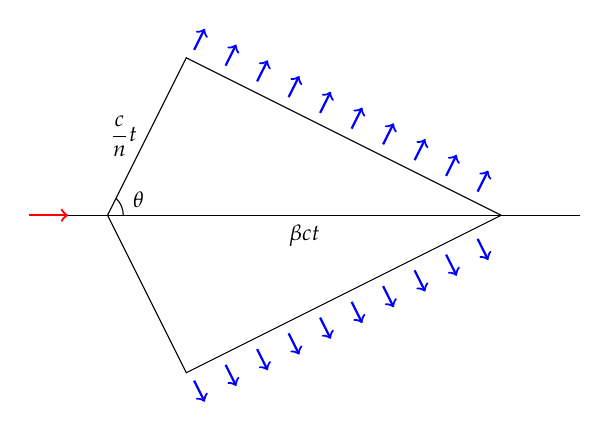
\begin{tikzpicture}
      \draw (-1,0) -- (6,0);
      \draw (0,0) -- (1,2) -- (5,0);
      \draw (0,0) -- (1,-2) -- (5,0);
      \draw[->, red, thick] (-1,0) -- (-0.5,0);
      \draw (0.2,0)arc[radius=.3,start angle=0,end angle=45];
      \node [left] at (0.5,1) {\footnotesize$\dfrac{c}{n}t$};
      \node [below] at (2.5 ,0) {\footnotesize$\beta c t$};
      \node [right] at (0.2,0.2) {\footnotesize$\theta$};
      \foreach \x in {0,1,...,9} {
        \draw[->,blue, thick] (1.1 + \x*0.4, 2.1 - \x*0.2)  --+ (63.435:0.3);
        \draw[->,blue, thick] (1.1 + \x*0.4, -2.1 + \x*0.2) --+ (-63.435:0.3);
      }
    \end{tikzpicture}
  \caption{Cherenkov radiation where $\theta$ is equal to $\cos\theta = \dfrac{\frac{c}{n}t}{\beta ct}$}
  \label{fig:label}
\end{figure}

\begin{align}
    x_p &= v_{p}\cdot t = \beta c t \nonumber \\
    x_{\text{em}} &= v_{\text{em}}\cdot t=\frac{c}{n}t \nonumber \\
    \cos\theta &= \frac{x_{\text{p}}}{x_{\text{em}}} = \frac{\frac{c}{n}t}{\beta c t} = \frac{1}{n\beta} \nonumber
\end{align}
which is independent of time.

\section{RICH detector} % (fold)
\label{sec:rich_detector}

Particle identification is a fundamental requirement at the LHC\textit{b} experiment. Meaningful CP-violation measurements are only possible if hadron identification is available hence the ability to distinguish between kaons and pions is  essential.
The LHC\textit{b} experiment is unique in the sense that its hadronic particle identification is handled only by the RICH sub-detectors. This means -- as mentioned before -- that the RICH has to cover a wide range of momentum (1-100 $\text{GeV}/c$).

Both sub-detectors are located in low magnetic field regions to keep the tracks straight while they pass through the radiators. They both 
also have a tilted spherical focusing primary mirror and a secondary flat mirror to limit the length of the detector along the beam pipe.

The RICH-1 in front of the magnet covers a lower momentum range from 1-60 $\text{GeV}/c$. It is composed of 5\,cm thick aerogel tiles arranged around the beam pipe. The aerogel with $n=1.03$ is suited for the lowest momentum tracks. Directly behind the aerogel is circa 1\,m of $\text{C}_4\text{F}_{10}$ which covers the intermediate region of momentum.
For the highest momentum tracks, gaseous $\text{C}\text{F}_4$ is used in the RICH-2.

There is a strong corelation between the polar angle and momentum of the tracks. Tracks with a wider angle often have lower momentum. That is why RICH-1 with the aerogel is located before the dipole magnet so tracks with low momentum will be covered before they swept out of the acceptenace by the magnet.

\begin{figure}[tb]
  \centering
  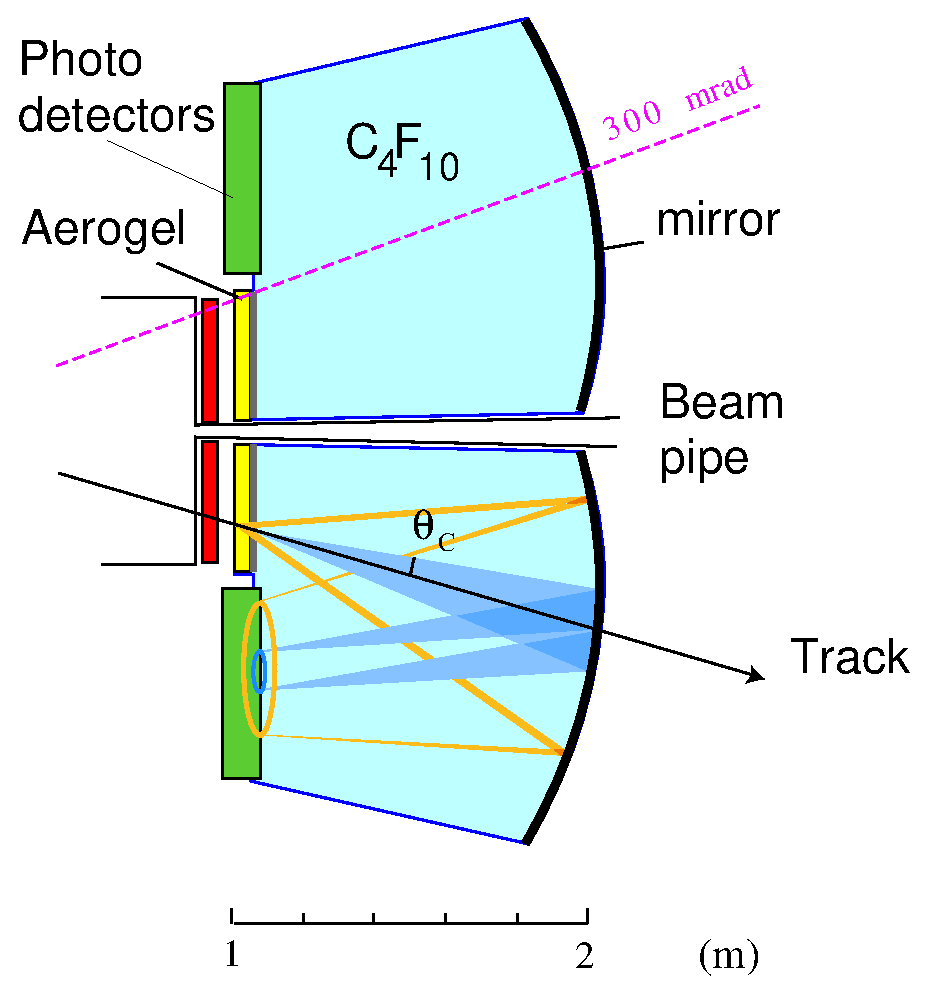
\includegraphics[width=0.5\textwidth]{pics/rich1_schematic}
  \caption{RICH-1 detector \cite{LHCb:2000}.}
  \label{fig:rich1}
\end{figure}
% section rich_detector (end)


% section cherenkov_radiation (end)

\section{Hough transform} % (fold)
\label{sec:hough_transform}

The Hough transform is a feature extraction technique used in image analysis, computer vision and digital image processing.

The purpose is to find imperfect instances of objects within a certain cass of shapes by a voting procedure. This voting procedure is carried out in a parameter space from which object candidates are obtained as local maxima in a so called accumlator space that is explicitly constructed by the algorithm for computing the Hough transform.

Initially the Hough transform was concerned with finding straight lines but has been extended to identifying positions of arbitrary shapes, such as circles and ellipses.

\subsection{Linear Hough transform} % (fold)
\label{sub:linear_hough_transform}

A linear function is normally defined as the following:

\[
  f(x) = m\cdot x + b
\]
where $m$ is the slope of the line and $b$ the intercept. For the Hough transform however, this representation is not ideal. For a vertical line $m$ would go to infinity which gives us an unbound transform space for $m$. For this reason Duda and Hart suggested the $\rho\text{-}\theta$ parametrization \parencite{Duda:1972}.

\begin{equation}
  r = x\cos\theta + y\sin\theta\label{eq:param_eq}
\end{equation}

where $r$ is the distance from the origin to the closest point in the line and $\theta$ is the angle between the $x$-axis and the line connecting the origin with that closest point.

\begin{figure}[ht]
  \centering
  \begin{tikzpicture}[scale=3]
    \draw[<->] (0,1.5) -- (0,0) -- (1.5,0);
    \draw[magenta,semithick] (0,1) -- (1,0);
    \draw[-> ,semithick] (0,0) -- (0.5, 0.5);
    \draw[semithick] (0.2,0) arc (0:45:0.2cm);
    \node[below] at (0.1,0.121) {\footnotesize$\rho$};
    \node[above] at (0.2,0.2) {$r$};
  \end{tikzpicture}
  \caption{$\rho\text{-}\theta$ parametrisation}
  \label{fig:rhotheta}
\end{figure}
% subsection linear_hough_transform (end)

This means given a single point in the plane, the set of all lines going through this point form a sinusoidal curve in $\rho\text{-}\theta$ space. Another point 
that lies on the same straight line in the plane will produce a sinusoidal curve that intersects with the other at ($\rho\text{-}\theta$) and so do all the points lying on the same straight line. 


\begin{figure}[tb]
  \centering
  \includegraphics[width=0.8\textwidth]{sim_pics/line_ht_paramspace}
  \caption[Example of a linear HT space]{Example of a linear HT parameter space. Each line is representing a point of the line. For each point several lines are drawn for different angles according to equation~\ref{eq:param_eq} so this plot draws the perpendicular distances from these lines to the origin. When different lines intersect it means that these 3 Points lie on a line with the parameters given by the plot.}
  \label{fig:line_ht}
\end{figure}

\begin{figure}[tb]
  \centering
  \includegraphics[width=0.8\textwidth]{sim_pics/line_ht_paramspace_nomatch}
  \caption[Example of a linear HT where points don't lie on a line]{Example of a linear HT where points don't lie on a line. Since any two points can form a line there are still intersections but never more than 2.}
  \label{fig:line_ht_nomatch}
\end{figure}

\subsection{Circle Hough transform} % (fold)
\label{sub:circle_hough_transform}

For this thesis we are interested in circle detection so we need to adapt our linear Hough transform in order to find circles. In a two dimensional space, a circle can be described by:

\begin{equation}
		(x-c_x)^2 + (y-c_y)^2 = r^2
\end{equation}

Where $(c_x,c_y)$ is the center of the circle and $r$ the radius. The possible parameters for the parameters space are now $c_x, c_y$ and $r$. This means if we know the center of the circle the parameter space is one-dimensional and if we know the radius of the circle our parameter space is two-dimensional and of course if we know nothing the parameter space is three-dimensional.



% subsection circle_hough_transform (end)
% section hough_transform (end)

\section{Dataset} % (fold)
\label{sec:dataset}
There are two data sets used for this thesis. One was the training data set of 250 events and then the data which tested the performance of the algorithm consisting of 10'000
individual events and a total of 49979 circles across all events. The properties of these events (radius, number of points per circle, number of circles per event) are taken from simulation and data.

The number of points per circle is determined by the photoelecton yield N$_\text{pe}$. It is measured for both \emph{normal} events and \emph{ideal}
events. The normal event is representative of nominal RICH running conditions during LHC\textit{b} physics detector operations. The ideal event is
a special event type with very low background hits \cite{RICHPerf2012}.

\begin{table}[tb]
\centering
\begin{tabular}{|c| c| c | c |c|}
\hline\hline
 & \multicolumn{2}{|c|}{N$_{\text{pe}}$ from data} & \multicolumn{2}{|c|}{N$_{\text{pe}}$ from simulation} \\ \hline
Radiator &  tagged D$^0 \rightarrow$ K$^- \pi^+$ &pp$ \rightarrow$ pp $\mu^+ \mu^-$ & Calculated $N_{\text{pe}}$ & true $N_{\text{pe}}$ \\ [0.5ex]
\hline
Aerogel & $5.0 \pm 3.0$  & $4.3 \pm 0.9$& $8.0 \pm 0.6$ & $6.8 \pm 0.3$ \\ \hline
C$_4$F$_{10}$  & $20.4 \pm 0.1$ & $24.5 \pm 0.3$& $28.3 \pm 0.6$ & $29.5 \pm 0.5$ \\ \hline
CF$_4$ & $ 15.8 \pm 0.1$  & $ 17.6 \pm 0.2$& $22.7 \pm 0.6$ & $23.3 \pm 0.5$ \\ 
\hline
\end{tabular}
\caption[Comparison of photoelectron yields (N$_{\rm pe}$)]{Comparison of photoelectron yields (N$_{\rm pe}$) determined from
D$^* \rightarrow$D$^0\pi^+$ decays in simulation and data, and 
pp $\rightarrow$ pp $\mu^+ \mu^-$ events in data, using the selections and 
methods described in the text \cite{RICHPerf2012}. The approximate value for 
C$_4$F$_{10}$ is between  $20.4 \pm 0.1$ and $29.5 \pm 0.5$ and for CF$_4$ between
$ 15.8 \pm 0.1$ and $23.3 \pm 0.5$ depending on the decay and whether it's the 
calculated value or the simulated value.}
\label{table:results}
\end{table}

\begin{figure}[tb]
  \centering
  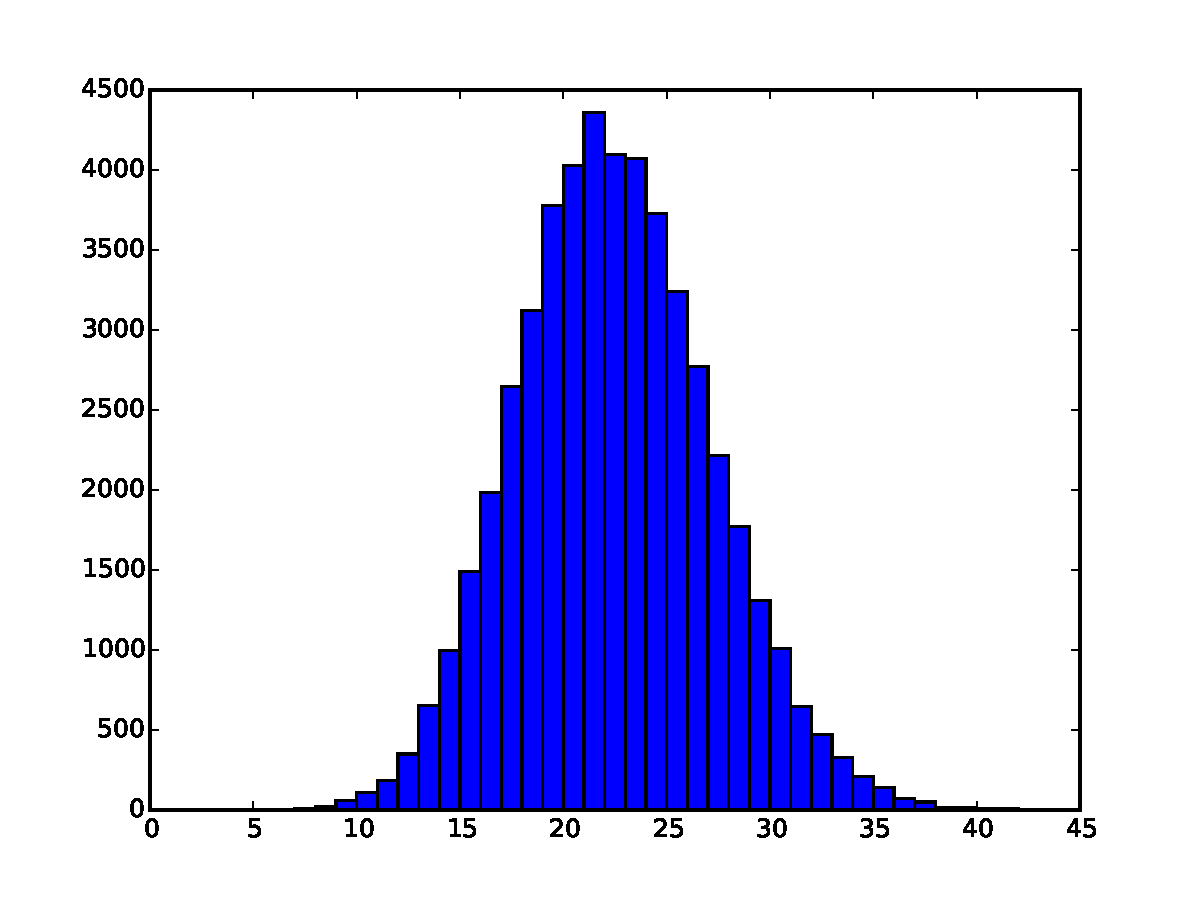
\includegraphics[width=0.6\textwidth]{sim_pics/ppc}
  \caption{Number of points per circle (N$_\text{pe}$) for the 10'000 events}
  \label{fig:ppc1}
\end{figure}

\begin{figure}[tb]
  \centering
  \includegraphics[width=0.6\textwidth]{sim_pics/circlePerEventDistribution}
  \caption{Number of circles per single event distribution.}
  \label{fig:circlePerEventDist}
\end{figure}

Also to get an idea what the average size of a Cherenkov ring is can be seen in
\cite{Forty1999}. Rings in RICH-1 have radiuses generally smaller than $0.15$\,m
(given they are from the C$_4$F$_{10}$ radiator; rings from the aerogel have
slightly bigger radiuses -- around $0.20$\,m). All the rings in the test data 
have a radius that is smaller than $0.15$\,m.

\begin{figure}[tb]
  \centering
  \includegraphics[width=0.6\textwidth]{sim_pics/radiusDist}
  \caption{The radius distribution of the test data events.}
  \label{fig:radius_dist}
\end{figure}
% section dataset (end)

\section{Existing algorithm} % (fold)
\label{sub:existing_algorithm}
There is already an algorithm in place in LHC\textit{b}. The disadvantage of the existing algorithm is due to the fact that it
uses tracks to reconstruct the circles. All charged tracks that are reconstructed by the tracking system are reflected at
the RICH mirrors in order to give a center for a Cherenkov ring. In order to match tracks with rings each ring is matched
with the track that has its position closest to the center of the ring. This means that this method uses information from
outside the RICH detector to construct the circles.

% subsection existing_algorithm (end)

\chapter{Methods}

\section{Conventional Hough transforms} % (fold)
\label{sec:conventional_hough_transforms}

In the following subsections we discuss the conventional Hough transforms for the case of a one, two and three dimensional parameter space. These
methods were mainly considered to get an idea what was possible with the conventional Hough transform. For closer study the method of choice was
the combinatorial triplet Hough transform discussed in depth in section \ref{sec:combinatorial_approach}.
% section conventional_hough_transforms (end)

\subsection{1D: Known center - find radius} % (fold)
\label{sub:1d_known_center_find_radius}

In this case the center(s) of the circle(s) is/are known so only the radius is missing. For the radius there is an array with a minimum value
and increasing by a defined stepsize to the maximum possible radius value. For the example in this thesis the minimum is $0$, the maximum radius
is $1$ and stepsize equal to $0.001$. Introducing following scoring function $\eta(r)$ allows to find the right radius.

\begin{equation}
\label{eq:score_function}
  \eta(r) = (c_x - x)^2 + (c_y - y) - r ^ 2
\end{equation}

and using this in a gauss distribution

\begin{equation}
\label{eq:weight_function}
  w(\eta) = \frac{1}{\sqrt{2\pi}\sigma}\exp\left( \frac{-\eta^2}{2\sigma^2}\right)
\end{equation}
\begin{figure}[tb]
  \centering
  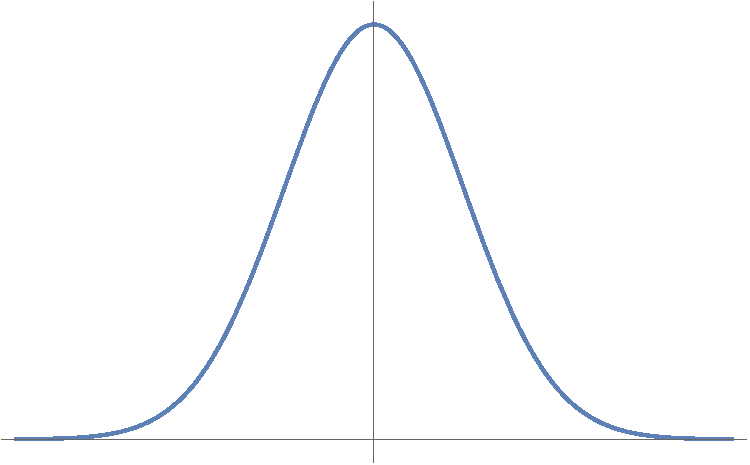
\includegraphics[width=0.5\textwidth]{pics/gauss}
  \caption[Normal Distribution: Used as a w`'eight function]{Using the probability density function of the normal distribution to calculate the score of a point in order to have a well defined maximum if a point
  lies directly on the circle and $\eta(r) = 0$. }
  \label{fig:gauss}
\end{figure}
Equation \ref{eq:weight_function} is of course just the circle equation with $c_x, c_y$ being the center of the circle, $x, y$ are the data points and $r$ the radius.
So if a lot of the data points have the same distance $r$ from the circle center there will be a high score for this particular radius. The index
for the highest score can then be used to find the corresponding radius.

\begin{figure}
  \begin{lstlisting}
  DMENSION = 1001
  r= linspace(0,1,DIMENSION)
  for c in centers:
    scores = zeros(DIMENSION)
    for x,y in allPoints:
      s = 2*BIN_WIDTH
      eta = (c_x-x)**2 + (c_y-y)**2 - r**2
      scores += 1. / ( sqrt( 2 * Pi ) * s ) 
                 * exp( -( eta ** 2 ) 
                  / ( 2 * s ** 2 ) )
    index = max(scores)
    circle = {}
    circle['center'] = c
    circle['radius'] = r[index]
\end{lstlisting}
\caption[Pseudo Code 1D HT]{Pseudo code for the 1D Hough transform. r is an array of length 1001 so $\eta$ will also be an 
array of length 1001. Scores is where the score for each iteration is stored. For each point the score is computed and added 
to the scores array and at the end the index with the highest score is the index we need to get the radius}
\end{figure}

\subsubsection{Complexity} % (fold)
The complexity of this algorithm is of $\mathcal{O}(n)$ where $n$ is the dimension of the radius array.
\label{ssub:complexity_1d}

% subsubsection complexity (end)

% subsection 1d_known_center_find_radius (end)
\subsection{2D: Known radius - find center} % (fold)
\label{sub:2d_known_radius_find_center}
Now the radius is known and the $x$ and $y$ coordinate of the center $(c_x, c_y)$ are unknown. Now instead of a one dimension the 
accumulator is 2 dimensional. The range of that space is simply the dimension of the plane which for this thesis is generally 
$[-0.5,0.5]$. Size of the bins is 0.001. So if the plane was 1\,m by 1\,m the accuracy of the accumulator in each dimension is 
up 1 mm. As in the one dimensional case we use the scoring function \ref{eq:score_function} in combination with the weight 
function \ref{eq:weight_function}.

\begin{figure}[b]
\begin{lstlisting}
  DIMENSION = 1001
  xbins = linspace(-0.5,0.5,DIMENSION)
  ybins = linspace(-0.5,0.5,DIMENSION)
  x, y = broadcast_arrays( xbins[..., newaxis], 
                           ybins[newaxis,...] )

  for r in Radiuses:
    weights = zeros( (DIMENSION,DIMENSION) )
    for xd,yd in allPoints:
      s = 2*BIN_WIDTH
      eta = (xd-x)**2 + (yd-y)**2 - r**2      
      weights += 1. / ( sqrt( 2 * pi ) * s ) 
                 * exp( -( eta ** 2 ) 
                 / ( 2 * s ** 2 ) )
    i, j = argmax(weights)
    removeUsedPoints()
    circle['Center'] = (xbins[i], ybins[j])
    circle['Radius'] = r
\end{lstlisting}
  \caption[Pseudo code 2D HT]{Pseudo code for the 2D Hough transform. xbins and ybins are arrays of length 1001. Here we use array broadcasting in order to avoid for loops and the weights can be evaluated in one line. This means that the x and y variables have dimension (1001,1001) but they don't take up that much memory. The x variable for example just broadcasts its value from the first row down to all the other rows and for y it broadcasts the first column to all the other columns. Weights variable is a 1001 by 1001 matrix. Again the entry with the highest score is the candidate for a possible circle center and if found stores in a final variable called circle.}
\end{figure}


\subsubsection{Complexity} % (fold)
\label{ssub:complexity_2d}
The complexity of this algorithm is $\mathcal{O}(n^2)$ where $n$ is the dimension of the histogram. The calculation of the weight has to be done for each data point of the 2D histogram. So in a $1000\times 1000$ histogram with 400 data points we calculate 400'000'000 times the weight of a grid point. Reducing the dimensions of the histogram weakens the accuracy of the whole algorithm but can speed up the calculations considerably. With a $1000\times 1000$ histogram the resolution in each space dimension is $1$\,mm. The RICH Technical Design Report states the resolution of the HPD is $2.5$\,mm $\times$ $2.5$\,mm.

The need (not entirely true) to calculate the weight for each grid point and data point means that there is a loop over data points and two loops for the $x$ and $y$ coordinate of the grid. To improve upon that there is the possibility of array broadcasting.
% subsubsection complexity (end)

\subsubsection{Array broadcasting}
Consider following one dimensional arrays where $x$ is a 1D histogram binning entries from 1 to 4 and same for $y$. 
\begin{align*}
  x &= [1, 2, 3, 4]\\
  y &= [1, 2, 3, 4]  
\end{align*}
Now all combinations between an element of $x$ and $y$ represent a 2D grid $\left((1,1), (1,2), ...\right)$. So to iterate through all those grid points one would have to create 2 for-loops iterating through $x$ and $y$

\noindent\begin{minipage}{\linewidth}
\begin{lstlisting}
def noBroadcast():
  a = np.random.randn(100)
  b = np.random.randn(100) 
  for x in a:
    for y in b:
      print (1-x)^2 + (2-y)^2 - 9
\end{lstlisting}  
\end{minipage}
%
This is not only slow but also doesn't look too nice if there are even more loops.
Broadcasting now turns this one dimensional array of length $n$ into an $n\text{ by }n$ matrix
\[
  x = \begin{bmatrix}
  1 & 1 & 1 & 1 \\
  2 & 2 & 2 & 2 \\
  3 & 3 & 3 & 3\\
  4 & 4 & 4 & 4
  \end{bmatrix}
\]
and
\[
  y = \begin{bmatrix}
  1 & 2 & 3 & 4 \\
  1 & 2 & 3 & 4 \\
  1 & 2 & 3 & 4 \\
  1 & 2 & 3 & 4 
\end{bmatrix}
\]
\noindent\begin{minipage}{\linewidth}
And with this the loops can be omitted:
\begin{lstlisting}
def withBroadcast():
  a = np.random.randn(100)
  b = np.random.randn(100) 
  x,y = np.broadcast_arrays(a[...,np.newaxis],
                            b[np.newaxis,...])
  print (1-x)^2 + (2-y)^2 - 9
\end{lstlisting}  
\end{minipage}
In this case this prints a $4$ by $4$ array with the function evualted for each combination of entries of $x$ and $y$
\[
  \begin{bmatrix}
    -8& -9& -8& -5\\
    -7& -8& -7& -4\\
    -4& -5& -4& -1\\
     1&  0&  1&  4
       \end{bmatrix}
\]
%
\begin{minipage}{\linewidth}
A runtime comparison shows   
\begin{lstlisting}
In [3]: %timeit withBroadcast()
10000 loops, best of 3: 76.8 us per loop

In [4]: %timeit noBroadcast()
100 loops, best of 3: 7.99 ms per loop
\end{lstlisting}
So the version with broadcasting is 100 times than the double loop. And the memory consumption is moderate since they broadcasted entries aren't new memory locations but just refer to the initial array.
\end{minipage}


\subsubsection{Optimizations} % (fold)
\label{ssub:optimizations}
It was mentioned before that for each data point the weight for the whole grid has to be calculated, that is not true. In the 2D case each grid point is a potential center for a circle only if it is not further a away and a threshold radius $R_T$, so if a grid point is further away than this threshold radius this calculation could be skipped. This could probably be done even smarter with the use of some sub grid so only points in the surrounding sub grids.

% subsubsection optimizations (end)

\subsubsection{Simple example of 2 circles without background} % (fold)
\label{ssub:simple_example_of_2_circles_without_background}
\begin{figure}[hp]
  \centering
  \includegraphics[width=0.5\linewidth]{sim_pics/2D_HT/center_scores_2_circles_0_bg_1}%
  \includegraphics[width=0.5\linewidth]{sim_pics/2D_HT/center_scores_2_circles_0_bg_2}

  \caption[2D weight matrix, first iteration]{(Left) 2D weight matrix in the first iteration of the Hough transform algorithm. (Right) Second iteration
  of the 2D weight matrix of the Hough transform. Points that satisfied the condition being less than a certain $\epsilon$ away from the radius found in the first iteration are removed leaving (hopefully) only points available that belong to the second circles}
  \label{fig:2d_weights_01}
\end{figure}
% subsubsection simple_example_of_2_circles_without_noise (end)
% section 2d_known_radius_find_center (end)

\subsection{3D: All parameters unknown} % (fold)
\label{sub:3d_nothing_is_known_find_everything}
In this section all that is known are the data points and the algorithm has to retrieve both center and radius of the circles. The accumulator space
is now in three dimensions. Two for the center coordinate and one for the radius. Similar as to the 2D case array broadcasting is used again
to speed up the calculations of the weight. Furthermore it is the first time that the algorithm has to decide itself whether or not all circles have
been found since there unlike in the previous two cases there isn't any information availabe about the circles so a condition has to be set
to decide when there are no more circles.
\begin{lstlisting}
xbins = np.linspace(-0.5,0.5,DIMENSION)
ybins = np.linspace(-0.5,0.5,DIMENSION)
rbins = np.linspace(0,0.5, R_DIMENSION)

x,y,r = np.broadcast_arrays(\
            xbins[np.newaxis,...,np.newaxis],\
            ybins[np.newaxis,np.newaxis,...],\
            rbins[...,np.newaxis,np.newaxis])
\end{lstlisting}
Broadcasting the $x,y,r$ arrays to speed up the calculations. To display the $x,y$ plane for a fixed radius it is important that rbins is
broadcast along the 2nd and 3rd axis. 
\begin{lstlisting}
while True:
  weights = np.zeros(\
         (R_DIMENSION, DIMENSION, DIMENSION))

  for x0,y0 in data['allPoints']:
    s = 0.001
    eta = (x-x0)**2 + (y-y0)**2 - r**2
    weights += 1./( sqrt( 2 * sconst.pi ) * s )*\
                      np.exp( -( eta ** 2 ) / \
                      ( 2 * s ** 2 ) )
  index = np.argmax( weights )
  rr,ii,jj = np.unravel_index( index, 
              (R_DIMENSION, DIMENSION, DIMENSION))
  score = weights[rr][ii][jj]
  if score < 2100:
    break  
\end{lstlisting}
As before a scoring function is used but this time the scoring function is of the form $f(x,y,r)$ and each point in weights then stands for the score of the
$x,y,r$ entries and their respective value.

Since there is now no information about any of the circles it is unknown how many circles there are so a condition is needed to stop looking for circles.
This algorithm uses a simple score threshold that whenever the highest score
of the weight matrix is less than a defined threshold the algorithm stops
and it is assumed that all circles have been found.
\begin{lstlisting}
circle['center'] = (xbins[ii], ybins[jj])
circle['radius'] = rbins[rr]
circles.append(circle)

used_xy += [tup for tup in data['allPoints'] if
    abs( ( tup[0] - circle['center'][0] ) ** 2 +
         ( tup[1] - circle['center'][1] ) ** 2 -
         circle['radius'] ** 2 ) < 2 * 0.001]
data['allPoints'][:] = 
            [tup for tup in data['allPoints'] if 
    abs( ( tup[0] - circle['center'][0] ) ** 2 + 
         ( tup[1] - circle['center'][1] ) ** 2 - 
         circle['radius'] ** 2 ) >= 2 * 0.001]  
\end{lstlisting}
Finally with the indices found the center and radius are retrieved
from the respective bins and saved to a circle dictionary. In order to
avoid finding the same circle twice or use data points twice a check
is being done to see whether a data point fulfills the requirement
of being a circle point. If that's the case that point will be put
into another list of already used points and the algorithm will not 
use this point anymore.
\subsubsection{Complexity} % (fold)
\label{ssub:complexity}
Assuming that the radius array has the same length as the two space
dimensions means that the complexity of this algorithm is of order 
$\mathcal{O}(N^3)$. As the 1D and 2D Hough transform the accuracy
directly depends on the binning. Same as for the 2D Hough transform
too match the resolution of the HPD of the RICH detector a binning of 400 makes sense if the detector dimensions are $1$\,m$\times1$\,m.
% subsubsection complexity (end)

\subsubsection{Optimisations} % (fold)
\label{ssub:optimisations}
As for the 2D HT introducing some kind of sub grid for the $x,y$ 
plane so only grid points in the vicinity of a data point are used
for calculating the score.
% subsubsection optimisations (end)
% subsection 3d_nothing_is_known_find_everything (end)

\section{Combinatorial triplet Hough transform}
\label{sec:combinatorial_approach}
A circle is uniquely defined by 3 points and radius and center can be calculated. If there are 15 points lying on the same circle there are 455 possible combinations of triplets According to the binomial distribution.
\[
   \binom{N}{3} = \frac{N!}{k!(N-k)!}
 \] 
Calculating the center and radius for these 455 triplets should result in the same center and same radius for all the triplets (floating point inaccuracy not considered). 

Having one background hit in addition to the 15 circle hits increases the triplet number to 560. The triplets with points solely consisting of points on the circle still have the same center and radius but the new combinations that now include a background hit will vary and it is unlikely that any two triplets that include the background point will have the same center and radius. Here is an overview of the algorithm used for this thesis.

\begin{enumerate}
\item Build all possible triples of points given the data points
\item For all the point triples calculate the center and the radius of the potential circle
\item Due to constraints in the radius many of the circles with a radius bigger than a certain threshold will be dropped.
\item Create a histogram with the radius distribution. Peaks in the radius distribution hint to a circle.
\item Scan the radius histogram for peaks and look at the center point histogram for the given radius of a peak. If there is also a peak in the center point histogram
      the set of the points of the triples lie on a circle with a radius and center given by the histogram peaks.
\end{enumerate}

\subsection{Generating the triples} % (fold)
\label{sub:generating_the_triples}
For generating the triples the built-in function \texttt{itertools.combinations()} of python is used. The input is an iterable, in our case a
list of tuples (each tuple is the $x$ and $y$ coordinate of a data point) which is used to create all possible combinations of triples (of said tuples).

% subsection generating_the_triples (end)

\subsection{Calculating the Circle given 3 points}

Let $(A,B,C)$ be a triple of points in a 2D plane and $a,b,c$ the length of the sides opposite to the respective corner.
%
The semiperimeter is defined as
%
\begin{equation}
  s = \frac{a+b+c}{2}
\end{equation}
%
using this we can calculate the radius $R$ of the circumcircle of triangle $\overline{ABC}$:
\begin{equation}
  R = \frac{abc}{4\sqrt{s(a+b-s)(a+c-s)(b+c-s)}}
\end{equation}
We have $\lambda_1, \lambda_2, \lambda_3$ as the barycenteric coordinates of the circumcenter:
\begin{align}
  \lambda_1 &= a^2\cdot(b^2+c^2-a^2)\\
  \lambda_2 &= b^2\cdot(a^2+c^2-b^2)\\
  \lambda_3 &= c^2\cdot(a^2+b^2-c^2)
\end{align}
Multiplying a matrix consisting of the column vectors of $A,B,C$ with a column vector of $\lambda_1, \lambda_2, \lambda_3$ and dividing the resulting vector by the sum of the barycentric coordinates (for noramlization) leads to the circumcenter of the triangle $\overline{ABC}$ 
%
\begin{equation}
  \begin{pmatrix}
    A_x & B_x & C_x \\
    A_y & B_y & C_y
  \end{pmatrix} \cdot \begin{pmatrix}
    \lambda_1\\
    \lambda_2\\
    \lambda_3
  \end{pmatrix} = \boldsymbol{P'}
\end{equation}
%
\begin{equation}
  \frac{\boldsymbol{P'}}{\lambda_1+\lambda_2+\lambda_3} = \boldsymbol{P}
\end{equation}
%
\begin{figure}[tb]
\centering
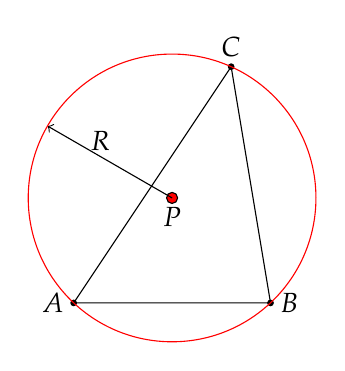
\begin{tikzpicture}
\coordinate (A) at (0,0);
\coordinate (B) at (2.5,0);
\coordinate (C) at (2,3);
\coordinate (Ci) at (1.25,1.33333);
\def\r{1.827}
\draw[thin] (A) -- (B) -- (C) -- cycle;
\node[left] at (A) {$A$};
\node[right] at (B) {$B$};
\node[above] at (C) {$C$};
\node[below] at (0.34,2.3) {$R$};
\draw[fill=black] (A) circle (1pt);
\draw[fill=black] (B) circle (1pt);
\draw[fill=black] (C) circle (1pt);
\draw[fill=red] (Ci) circle (2pt) node [below] (Ci) {$P$};

\draw[->] (1.25,1.33333) -- +(150:1.827);
\draw[red] (1.25,1.33333) circle (1.827);
\end{tikzpicture}
\caption{The circumradius ($R$) and the circumcenter ($P$) of a circle defined by three points.}
\label{fig:circum_fig}
\end{figure}



\subsection{Drawback}
	

There is also a drawback with this method: the combinatorics blow up with a high number of data points \( \binom{N}{3} \). So for example with 200 data points (circle data and background) the number of triplets is

\[ \binom{200}{3} = 1313400 \]
and for 300:
\[ \binom{300}{3} = 4455100 \]

So the complexity of the algorithm is roughly in the order of $\mathcal{O}(N^3)$ which can be easily seen when taking the upper bound of $\binom{N}{k} \leq \frac{N^k}{k!}$ and since $k=3$ then means $\frac{N^3}{3!}$ see figure \ref{fig:binom_growth}. 
\begin{figure}[ht]
\centering
  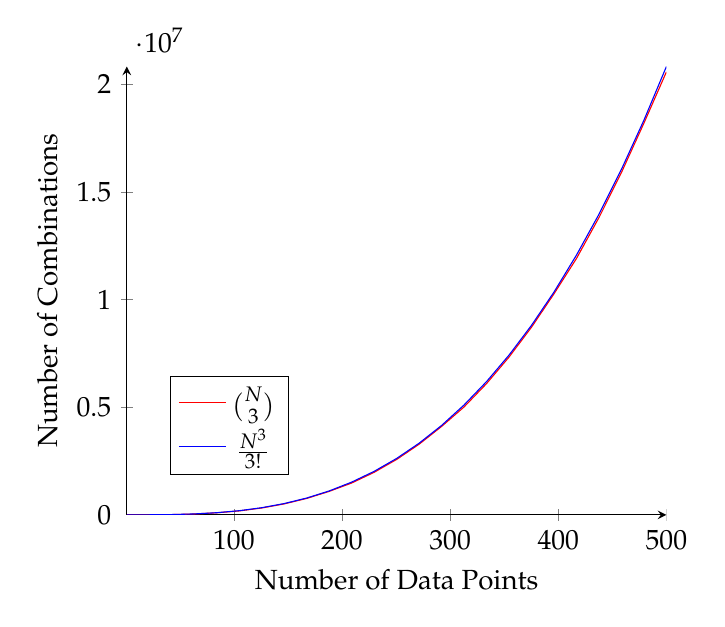
\begin{tikzpicture}
    \begin{axis}[
    axis lines = left,
    xlabel = Number of Data Points,
    ylabel = {Number of Combinations},
    legend style={at={(0.3,0.2)},anchor=east},
    ]
    \addplot [
    domain=1:500, 
    color=red,
    ]
    { factorial(x)/(factorial(x-3)*factorial(3))};
    \addplot [
    domain=1:500, 
    color=blue,
    ]
    { x^3/factorial(3)};
    \addlegendentry{$\binom{N}{3}$}
    \addlegendentry{$\frac{N^3}{3!}$}
    \end{axis}

  \end{tikzpicture}
    \caption[Complexity of the combinatorial triplet Hough transform]{Scaling of the algorithm. Binomial Growth with $\binom{N}{3}$ compared with the approximation $\frac{N^3}{3!}$. So the algorithm runs in the order of $\mathcal{O}(n^3)$}
  \label{fig:binom_growth}
\end{figure}


\subsubsection{Optimisation} % (fold)
\label{ssub:improvement_of_speed}

As seen before this approach scales with $\binom{N}{3}$. This means that with 500 data points we have to create around 20 million triplets which are used for calculating radiuses and centers of circles. 
To qualify as a circle the algorithm needs a threshold to decide if a candidate is a circle or not. The threshold is defined as such that the minimum amount of points/circle has to be $N$ in order to be considered as a circle candidate. This means that the threshold value is $\binom{N}{3}$. This of course means that circles with less than $N$ points will normally never be found unless another point that actually doesn't belong to the circle lies on the circle and contributes to the radius and center histogram pushing the circle above the threshold.

But not only the amount of triplets generated is a speed bump for the runtime but also the creation of this triplets takes about $\frac{N^3}{3!}$ time. So if there was a way to improve not only the amount of total triplets but also the time needed
to create them it would speed up the algorithm considerably.

This leads to the following idea: to split the original data set randomly into two lists. For each of these lists all the possible combinations of triplets is generated again and combined in one total list.

\begin{figure}[b]
\centering
  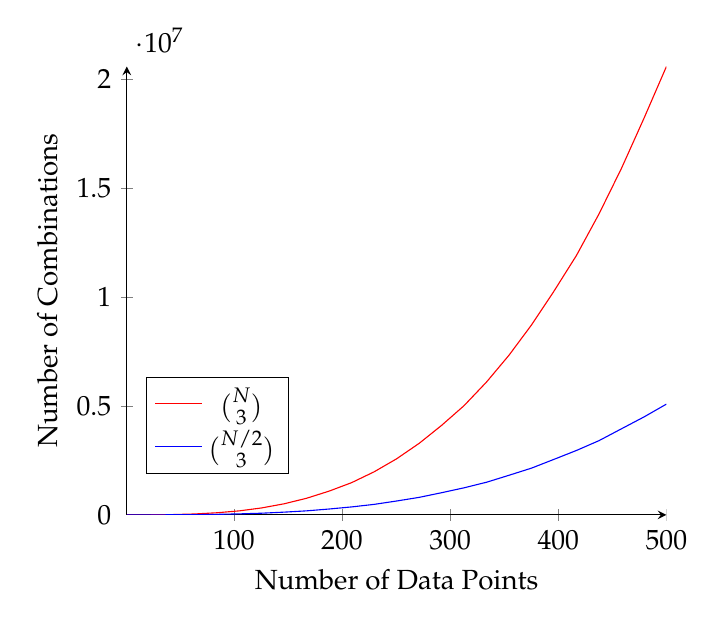
\begin{tikzpicture}
    \begin{axis} [
      axis lines = left,
      xlabel = Number of Data Points,
      ylabel = {Number of Combinations},
      legend style={at={(0.3,0.2)},anchor=east},
    ]
    \addplot [
    domain=1:500, 
    color=red,
    ]
    { factorial(x)/(factorial(x-3)*factorial(3))};
    \addplot [
    domain=1:500, 
    color=blue,
    ]
    { 2*factorial(x/2)/(factorial(x/2-3)*factorial(3)) };
        \addlegendentry{$\binom{N}{3}$}
    \addlegendentry{$\binom{N/2}{3}$}
    \end{axis}
  \end{tikzpicture}
  \caption{Number of combinations with $\binom{N}{3}$ compared to the number of combinations generated from $\binom{N/2}{3}$}
  \label{fig:binom_half_growth}
\end{figure}

The problem with this approach is the possible loss of information. Since the
algorithm has the threshold that defines how many entries a bin in the 
center histogram must have in order to be accepted as a radius/circle center.
This threshold should be high enough that triplets that contain noise points
do not contain to the circles but low enough that real circles with low point
can still be found.
\begin{figure}[tb]
   \centering
   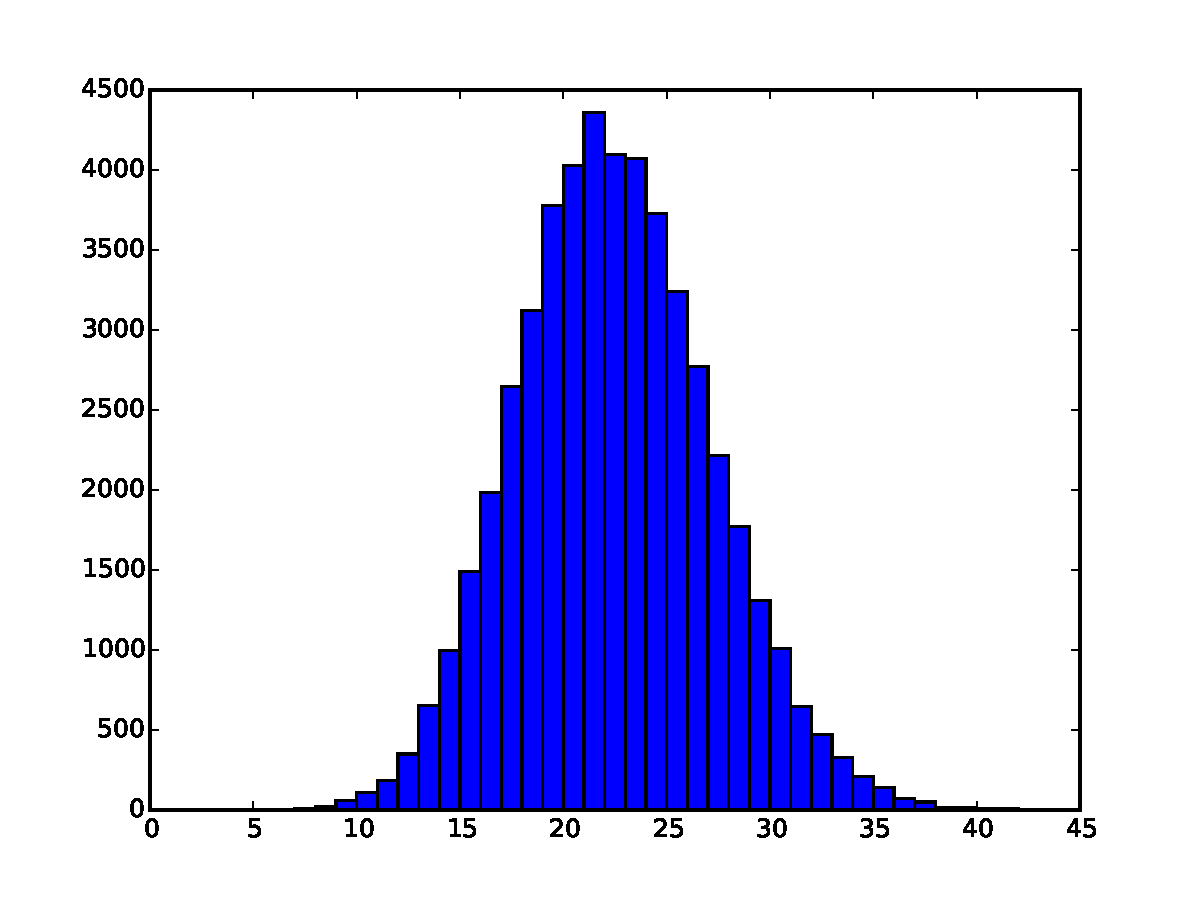
\includegraphics[width=0.8\textwidth]{sim_pics/ppc}
   \caption{Distribution of points per circle. }
   \label{fig:ppc}
 \end{figure} 


If now the data is randomly split in two lists there are only 2 ways where
a circle with 10 hits will still be found namely that all the 10 points end
up in the same half of the list.
  \begin{table}[tb]
  \centering
  \caption{Example of ways to split points into 2 lists.}
    \label{tab:point_split}
  \begin{tabular}{cc}
  \toprule
  \textbf{Pts in list 1} & \textbf{Pts in list 2} \\
  \midrule
     10 & 0 \\
     9  & 1 \\
     8  & 2 \\
     $\vdots$ & $\vdots$ \\
     2 & 8\\
     1 & 9\\
     0 & 10 \\
  \bottomrule
  \end{tabular}

\end{table}

So the question is what are the probabilities that splitting a data set with
10 or more points ends up with 1 list having more than 10 points. As soon as
a circle has 20 points this becomes moot as always one list will have more 
than 10 points (see Figure~\ref{fig:ratios}).

From figure~\ref{fig:ratios} it is clear that even if we split the lists there is a more 
than 50\% chance that we lose no information once a circle has 13 points.
\begin{figure}[htb]
  \centering
  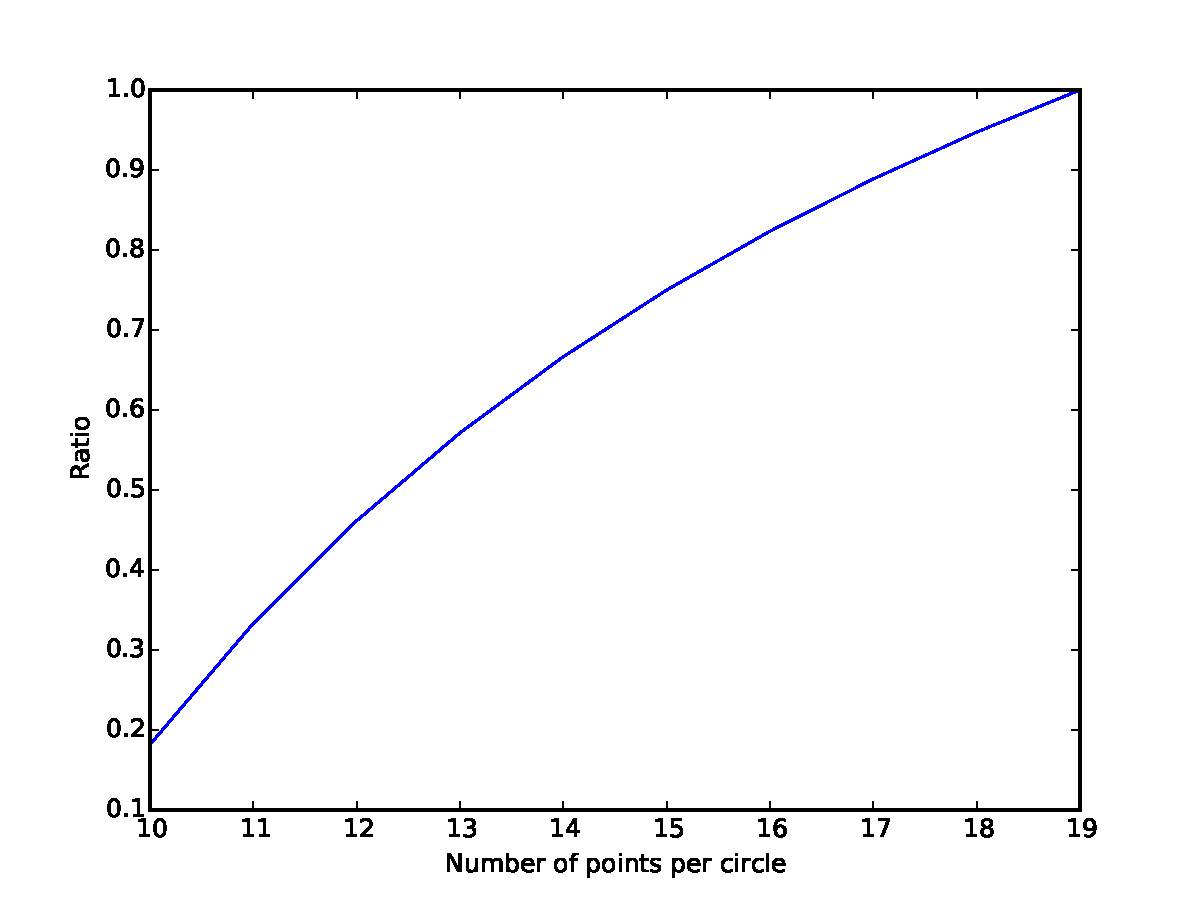
\includegraphics[width=\textwidth]{pics/ratio.pdf}
  \caption{The probability when splitting randomly a list of $x$ points into two that one list has more than 10 points.}
  \label{fig:ratios}
\end{figure}

% subsubsection optimisation (end)

\subsection{Possible optimisation: average radius of random circles in a unit square} % (fold)
\label{ssub:average_radius_of_random_circles_in_a_unit_square}
An interesting property of calculating the radius of triplets generated from points that are distributed uniformely in the unit square is 
that they always obey a certain shape.

To prove this the expected area of a triangle formed by three points randomly chosen from the unit square\footnote{This proof is taken
from \cite{Blatter:2015}} has to be calculated. Let \( A = (a_1, a_2),\ B = (b_1, b_2),\ C = (c_1, c_2)\) be the vertices of the random triangle \( T \). We consider the case where \( a_2
> b_2 > c_2 \) which takes $\frac{1}{6}$ of the total ``Volume''. Fix \( a_2, b_2, c_2 \) for the moment and we can write.
\[
  b_2 = (1-t)a_2 + tc_2, \qquad 0 \leq t \leq 1.
\]
The side $AC$ of $T$ intersects the horizontal level $y=b_2$ at the point $S=(s,b_2)$ with
\begin{equation}
  s = s(a_1,c_1,t) = (1-t)a_1 + tc_1
\end{equation}
The area $X$ of $T$ is then given by
\[
  X = \frac{1}{2}\lvert b_1 - s\rvert(c_2 - a_2)
\]
We now start integrating with respect to our six variables. The innermost integral is with respect to $b_1$ and gives

\begin{align}
  X_1 &:= \int_0^1X\text{d}b_1=\frac{1}{2}(c_2-a_2)\left( \int_0^s(s-b_1)db_1 + \int_s^1(b_1-s)db_1\right)\nonumber\\
      &\phantom{:}= \frac{1}{4}(c_2-a_2)(1+2s+2s^2)\nonumber
\end{align}
Next we integrate over $b_2$:
\begin{align}
  X_2 &:= \frac{1}{4}\int_0^1\int_{a_2}^1(c_2-a_2)^2\,dc_2\,da_2\,\times\,\int_0^1\int_0^1\int_0^1(1-2s+2s^2)\,dt\,dc_1\,da_1  \nonumber
\end{align}
This gives
\[
  X_3 = \frac{1}{4}\cdot \frac{1}{12} \cdot \frac{11}{18} = \frac{11}{6\cdot144}
\]
But generalizing our assumption at the beginning $a_2 < b_2 < c_2$ we multiply this result by $6$ and obtain then $\frac{11}{144}$.

From \cite{Weisstein2016} follows that the average area of a triangle in a unit circle is $\frac{3}{2\pi}$ so dividing this area by the
area of the unit circle gives the expected area covered by a triangle in an arbitrary circle

\[
\frac{\text{Expected area of a triangle in a unit circle}}{\text{Area of the unit circle}} = \underbrace{\frac{\frac{3}{2\pi}}{\pi r^2}}_{r=1} = \frac{3}{2\pi^2}
\]

So finally the average area of a random circle can be obtained by dividing the average area of a triangle from the unit square by expected
area covered by a triangle in an arbitrary circle so essentially the average area of a random circle within the unit square:

\[
  \frac{\frac{11}{144}}{\frac{3}{2\pi^2}} = \frac{11\pi^2}{216}
\]

This should be equal to $\pi R^2$ where $R$ is the average radius of a random circle in the unit cube

\begin{align}
  R\pi^2 &= \frac{11\pi^2}{216}\nonumber\\
  R &= \sqrt{\frac{11\pi}{216}} = 0.399986\nonumber
\end{align}

Generating a random background and then plotting the radius histogram for this data set shows that there is indeed a peak around
 $R\approx 0.4$.

 \begin{figure}[tb]
   \centering
   \includegraphics[width=0.8\textwidth]{sim_pics/background_radius_for_diff_background}
   \caption[Radius distribution for background]{Radius distribution for uniformly generated background. The expected value of $R\approx 0.4$
   is quite well represented for differently sized data sets}
   \label{fig:rad_dist}
 \end{figure}

% subsubsection average_radius_of_random_circles_in_a_unit_square (end)
% chapter methods (end)
\chapter{Results}
\label{cha:results}
In this section results for the conventional 1D, 2D, 3D Hough transform and the combinatorial triplet Hough transform are presented. 1D and 2D Hough transform
were not pursued in depth. Nonetheless they are presented here as they offer a nice
way of understanding how each extra dimension expands the algorithm and also
shows the flaws with each added dimension.

For the 1D and 2D Hough transform very simple data data was used. There were 
no physical constraints when generating the circles and their point/circle
or also their radius distribution doesn't reflect the real data obtained
by LHC\textit{b}.

\section{1D Hough transform results} % (fold)
\label{sec:1d_hough_transform_results}
For this section following different data sets were tested.
\begin{itemize}
  \item 1 circle and 600 background hits
  \item 2 circles and 0 background hits
  \item 5 circles and 30 background hits
\end{itemize}

For each set the radius score is shown and the final result of the algorithm.
The algorithm has no problems to find any of the circles even with background.
But this was expected as the algorithm only needs to search in one dimension
and makes the whole process very easy.

\subsection{Overview of the results} % (fold)
\label{sub:1d_overview_of_the_results}
First an overview about different test cases. The event with 1 circle and 600
background hits means to test how robust the algorithm is with a lot of
background hits. The second test case means to test if the algorithm can 
handle two circle objects and the third event is a mix between several
circles and some background hits.

There is are different plots
\begin{itemize}
  \item Radius score
  \item Resulting circle
\end{itemize}

The radius score is a 1D plot of the weight function $f(r)$~\ref{eq:weight_function}. The highest peak
indicating the maximum score and its location telling the value of the radius.
The resulting circle plot is the center (which was known) and the extracted radius combined, drawing the resulting circle. There is always the same plot
again with center and radius taken directly from data to compare the two results.

% subsection overview_of_the_results (end)
\begin{figure}[htp]
        \centering
        \subfloat[][1 circle, 600 background hits. \label{fig:1c600bg}]{\includegraphics[width=0.3\textwidth]{sim_pics/1D_HT/result_1_circle_600_bg}}
        ~ %add desired spacing between images, e. g. ~, \quad, \qquad etc.
          %(or a blank line to force the subfigure onto a new line)
       \subfloat[][2 circles, 0 background hits]{\includegraphics[width=0.3\textwidth]{sim_pics/1D_HT/result_2_circles_0_bg}}
                \label{fig:2c0bg}
        ~ %add desired spacing between images, e. g. ~, \quad, \qquad etc.
          %(or a blank line to force the subfigure onto a new line)
        \subfloat[][5 circles, 30 background hits]{\includegraphics[width=0.3\textwidth]{sim_pics/1D_HT/result_5_circles_30_bg}}
                \label{fig:5c30bg}
        \caption{Circles found by the 1D Hough transform. The circle in Figure~\ref{fig:1c600bg} has its center in the origin so the algorithm did find the circle.}\label{fig:1d_ht_results}

        \subfloat[][1 circle, 600 background hits.]{\includegraphics[width=0.3\textwidth]{sim_pics/1D_HT/real_result_1_circle_600_bg}}
                \label{fig:real_1c600bg}
        ~ %add desired spacing between images, e. g. ~, \quad, \qquad etc.
          %(or a blank line to force the subfigure onto a new line)
        \subfloat[][2 circles, 0 background hits]{\includegraphics[width=0.3\textwidth]{sim_pics/1D_HT/real_result_2_circles_0_bg}}
                \label{fig:real_2c0bg}
        ~ %add desired spacing between images, e. g. ~, \quad, \qquad etc.
          %(or a blank line to force the subfigure onto a new line)
        \subfloat[][5 circles, 30 background hits]{\includegraphics[width=0.3\textwidth]{sim_pics/1D_HT/real_result_5_circles_30_bg}}
                \label{fig:real_5c30bg}
        \caption{These are the circles as generated by the simulation. All of these examples were correctly solved by the 1D Hough transform.}\label{fig:real_1d_ht_results}
\end{figure}

\subsection{1D Hough transform - 2 circles, 0 background hits} % (fold)
\label{sub:1d_hough_transform_2_circles_0_background}
Two circle objects have to be found in this event with zero background.
% subsection 1d_hough_transform_2_circles_0_background (end)
\begin{figure}[htp]
        \subfloat[][1 circle, 600 background hits.]{\includegraphics[width=0.5\textwidth]{pics/1D_HT/radius_scores_2_circles_0_bg_1}}
                \label{fig:2c0bg_radius1}
        \subfloat[][2 circles, 0 background hits]{\includegraphics[width=0.5\textwidth]{pics/1D_HT/radius_scores_2_circles_0_bg_2}}
                \label{fig:2c0b_radius2}
        \caption{Radius score for the 1D Hough transform for 2 circles with 0 background. The respective radiuses are $0.191$ and $0.108$ }\label{fig:1d_ht_radius}
\end{figure}
Each peaks is clearly visible in their respective radius score plots. The algorithm has no problems finding two distinct circles in the plane.
If two circles had the same radius and their centers are also the same (unlikely) then the algorithm in its current state would find only one circle.
A way around this could be introducing a maximum score that when a certain score is exceeded then the algorithm assumes it's more than just 1 circle.
But if both circles have a low number of points this still might fail. So all in all it is not fool proof.

\subsection{1D Hough transform - 5 circles, 30 background hits} % (fold)
\label{sub:1d_hough_transform_5_circles_30_background_hits}
In figure~\ref{fig:5_circles_30_bg_radius} the different radius scores for each known center are shown. The algorithm calculates 
the score for one center with all data points at a time and the radius with the highest score gets assigned to that center.
Once done for all centers the algorithm is done.
\begin{figure}[ht!]
  \centering
  \subfloat{\includegraphics[width=0.5\textwidth]{sim_pics/1D_HT/result_5_circles_30_bg}}
  \subfloat{\includegraphics[width=0.5\textwidth]{sim_pics/1D_HT/real_result_5_circles_30_bg}}
  \caption[5 circles, 30 background hits result]{The result for 5 circles with 30 background hits. On the left the result obtained by 
  the 1D Hough transform algorithm while the circles from the simulated data is on the right.}
  \label{fig:1d_5c_30bg}
\end{figure}

\begin{figure}[htbp]
\centering
  \subfloat{\includegraphics[width=0.5\textwidth]{sim_pics/1D_HT/radius_scores_5_circles_30_bg_1}}
  \subfloat{\includegraphics[width=0.5\textwidth]{sim_pics/1D_HT/radius_scores_5_circles_30_bg_2}}
  
  \subfloat{\includegraphics[width=0.5\textwidth]{sim_pics/1D_HT/radius_scores_5_circles_30_bg_3}}
  \subfloat{\includegraphics[width=0.5\textwidth]{sim_pics/1D_HT/radius_scores_5_circles_30_bg_4}}

  \subfloat{\includegraphics[width=0.5\textwidth]{sim_pics/1D_HT/radius_scores_5_circles_30_bg_5}}
  \caption{1D HT: Radius scores for all the centers for an event with 5 circles. The noise contributes only very little to the radius peaks
  and identifying the circle candidates is easy.}
  \label{fig:5_circles_30_bg_radius}
\end{figure}
As exptected the circles can be reconstructed.

% subsection 1d_hough_transform_5_circles_30_background_hits (end)


% section 1d_hough_transform_results (end)
\newpage
\section{2D Hough transform results} % (fold)
\label{sec:2d_hough_transform_results}
The 2D Hough transform searches in the $x,y$ space for suitable
circle centers that have a high score. The same events as for the 1D
Hough transform were investigated to make a comparison about reliability.
In a first overview the algorithm performs quite well and finds all the
circles.

These were some of the events tackled by the algorithm (among others).
\begin{itemize}
  \item 1 circle and 600 background hits
  \item 2 circles and 0 background hits
  \item 5 circles and 30 background hits
\end{itemize} 
and additionally
\begin{itemize}
  \item 6 circles and 200 background hits
\end{itemize}

\subsection{Overview of the results} % (fold)
\label{sub:2d_overview_of_the_results}
As in subsection \ref{sub:1d_overview_of_the_results} in a first step an overview of the results. The same events as before but this time tested with the 2D
Hough transform. All the circles were found correctly but the example with 6 circles and 200 background hits shows that the algorithm can fail to find a 
circle. The reason is quite simple. Both, the yellow and magenta circle, have similar radiuses. Now the algorithm looks first for the magenta circle (because that happens to be the way the centers are arranged in the list) and since so many points of the yellow circle lie so close together it is easy for the magenta circle (who has a similar radius) to get a high score with these points, a higher score than it would get with its proper points. If the yellow points were more evenly distributed on the circle or if there were more magenta points this probably wouldn't happen but that is something that can't be controlled.
% subsection overview_of_the_results (end)

\begin{figure}[htp]
        \centering
        \subfloat[][1 circle, 600 background hits. The circle is centered at $0.0/0.0$. \label{fig:2d_1c600bg}]{\includegraphics[width=0.3\textwidth]{sim_pics/2D_HT/result_1_circle_600_bg}}
        ~ %add desired spacing between images, e. g. ~, \quad, \qquad etc.
          %(or a blank line to force the subfigure onto a new line)
        \subfloat[][2 circles, 0 background hits\label{fig:2d_2c0bg}]{\includegraphics[width=0.3\textwidth]{sim_pics/2D_HT/result_2_circles_0_bg}}
        ~ %add desired spacing between images, e. g. ~, \quad, \qquad etc.
          %(or a blank line to force the subfigure onto a new line)
        \subfloat[][5 circles, 30 background hits  \label{fig:2d_5c30bg}]{\includegraphics[width=0.3\textwidth]{sim_pics/2D_HT/result_5_circles_30_bg}}
              
        \caption{Circles found by the 2D Hough transform.}\label{fig:2D_HT_results1}

        \subfloat[][1 circle, 600 background hits.\label{fig:2d_real_1c600bg}]{\includegraphics[width=0.3\textwidth]{sim_pics/2D_HT/real_result_1_circle_600_bg}}
        ~ %add desired spacing between images, e. g. ~, \quad, \qquad etc.
          %(or a blank line to force the subfigure onto a new line)
        \subfloat[][2 circles, 0 background hits]{\includegraphics[width=0.3\textwidth]{sim_pics/2D_HT/real_result_2_circles_0_bg}}
                \label{fig:2d_real_2c0bg}
        ~ %add desired spacing between images, e. g. ~, \quad, \qquad etc.
          %(or a blank line to force the subfigure onto a new line)
        \subfloat[][5 circles, 30 background hits]{\includegraphics[width=0.3\textwidth]{sim_pics/2D_HT/real_result_5_circles_30_bg}}
                \label{fig:2d_real_5c30bg}
        \caption{The circles as generated by the simulation. All of these examples were correctly solved by the 2D Hough transform.}\label{fig:real_2d_ht_results2}

        \subfloat{\includegraphics[width=0.5\textwidth]{sim_pics/2D_HT/result_6_circles_200_bg}}
        \subfloat{\includegraphics[width=0.5\textwidth]{sim_pics/2D_HT/real_result_6_circles_200_bg}}
        \caption{Circles found by the algorithm on the left and the correct results on the right. The magenta colored circle in the left image is incorrect. It replaced
        the yellow circle (taken from the simulated data on the right).}
        \label{fig:2d_6c_200_bg}
\end{figure}

Theoretically it is also possible that the yellow circle gets fitted to the
magenta points but since there are still enough yellow points left after the removal of the points assigned to the magenta circle they still have the highest score with their own points and the magenta circle goes unnoticed.

Also, if the yellow circle would be checked before magenta then the algorithm
would find the proper circles as well. So it actually can depend on the order
in which the circles are searched.

\subsection{2D Hough transform, 2 circles, 0 background hits} % (fold)
\label{sub:2d_hough_transform_2_circles_0_background}
Two circle objects have to be found in this event with zero background. This
poses no problem unless the two circles have the same radius then without
removing points that have been used for one circle it will always find the 
circle with the higher score. Introducing a mechanism that removes points
that were assigned to a circle solves this problem.

\begin{figure}[htp]
        \centering
        \subfloat{\includegraphics[width=0.5\textwidth]{sim_pics/2D_HT/center_scores_2_circles_0_bg_1}}
        \subfloat{\includegraphics[width=0.5\textwidth]{sim_pics/2D_HT/center_scores_2_circles_0_bg_2}}
        \caption{Center score for the 2D Hough transform for 2 circles with 0 background.}\label{fig:2d_ht_center}

        \includegraphics[width=0.5\textwidth]{sim_pics/2D_HT/projection/stacked_projection_9_2}%
        \includegraphics[width=0.5\textwidth]{sim_pics/2D_HT/projection/stacked_projection_9_1}
        \caption[Two slices out of the 2D histogram]{Two slices out of the 2D histogram. These 2D histograms are very similar to the radius histogram from the 1D HT
        but now instead of the weights for the radius which is 1 dimensional the weights for $x,y$ are calculated which are
        2 dimensional}

        \subfloat{\includegraphics[width=0.5\textwidth]{sim_pics/2D_HT/result_2_circles_0_bg}}
        \subfloat{\includegraphics[width=0.5\textwidth]{sim_pics/2D_HT/real_result_2_circles_0_bg}}
\caption[Results of 2D HT, 2 circles, 0 background]{2D HT: Although already shown before for completeness the 2 circle 2D Hough transform result. Left side the result from the algorithm on the right side the correct result from data.}
\end{figure}

% subsection 2d_hough_transform_2_circles_0_background (end)

\subsection{2D Hough transform, 5 circles, 30 background hits} % (fold)
\label{sub:2d_hough_transform_5_circles_30_background_hits}

This event added more circles but also some background hits. Both were handled
well by the algorithm and all the circles were found.

\begin{figure}[htbp]
  \centering
  \subfloat{\includegraphics[width=0.5\textwidth]{sim_pics/2D_HT/center_scores_5_circles_30_bg_1}}
  \subfloat{\includegraphics[width=0.5\textwidth]{sim_pics/2D_HT/center_scores_5_circles_30_bg_2}}
  
  \subfloat{\includegraphics[width=0.5\textwidth]{sim_pics/2D_HT/center_scores_5_circles_30_bg_3}}
  \subfloat{\includegraphics[width=0.5\textwidth]{sim_pics/2D_HT/center_scores_5_circles_30_bg_4}}
  
  \subfloat{\includegraphics[width=0.5\textwidth]{sim_pics/2D_HT/center_scores_5_circles_30_bg_5}}
  \caption{Center scores for all the centers for an event with 5 circles.}
  \label{fig:2d_5_circles_30_bg_radius}
\end{figure}
\begin{figure}
\centering
  \subfloat{\includegraphics[width=0.5\textwidth]{sim_pics/2D_HT/result_5_circles_30_bg}}
  \subfloat{\includegraphics[width=0.5\textwidth]{sim_pics/2D_HT/real_result_5_circles_30_bg}}
  \caption{The reconstructed result on the left while the circles from the simulated data is on the right.}
  \label{fig:2d_5c_results}
\end{figure}
% subsection 2d_hough_transform_5_circles_30_background_hits (end)

\subsection{2D Hough transform, 6 circles, 200 background hits} % (fold)
\label{sub:2d_hough_transform_6_circles_200_background_hits}
As briefly discussed in the overview the algorithm does make mistakes as this event will show. 6 circles 
were generated with 200 background hits. The interesting part is not that amount of circles or the amount
of background hits are the problem but the properties of the circles (center coordinate and radius). In 
this example there is a misidentification of a circle with points of another.
% subsection 2d_hough_transform_6_circles_200_background_hits (end)

\begin{figure}
\centering
  \subfloat{\includegraphics[width=0.3\textwidth]{sim_pics/2D_HT/center_scores_6_circles_200_bg_1}}
  \subfloat{\includegraphics[width=0.3\textwidth]{sim_pics/2D_HT/center_scores_6_circles_200_bg_2}}
  \subfloat{\includegraphics[width=0.3\textwidth]{sim_pics/2D_HT/center_scores_6_circles_200_bg_3}}

  \subfloat{\includegraphics[width=0.3\textwidth]{sim_pics/2D_HT/center_scores_6_circles_200_bg_4}}
  \subfloat{\includegraphics[width=0.3\textwidth]{sim_pics/2D_HT/center_scores_6_circles_200_bg_5}}
  \subfloat{\includegraphics[width=0.3\textwidth]{sim_pics/2D_HT/center_scores_6_circles_200_bg_6}}
  \caption[Center scores for 6 circles with 200 background hits.]{Center scores for 6 circles with 200 background hits. There is a lot more going on because of all the background hits that by accident contribute to a high score all over the grid.}

  \subfloat{\includegraphics[width=0.5\textwidth]{sim_pics/2D_HT/result_6_circles_200_bg}}
  \subfloat{\includegraphics[width=0.5\textwidth]{sim_pics/2D_HT/real_result_6_circles_200_bg}}
\caption{On the left side the wrong result obtained by the 2D Hough transform and the correct one on the right side}
\end{figure}

A possible way to fix this particular problem is to tune the parameters of the weight function namely reducing the standard deviation. 
\[
  w(\eta) = \frac{1}{\sqrt{2\pi}\sigma}\exp\left( \frac{-\eta^2}{2\sigma^2}\right)
\]
Having a higher $\sigma$ means that a point that is a bit off of the circle still contributes a considerable value to the total score. The smaller the $\sigma$ is the sharper the peak. However if the peak is too sharp then the algorithm might discard possible results because they are just a bit off the circle but since the peak is so narrow they don't contribute at all to the total score.

In the example before $\sigma$ was equal to $0.001$ while the space dimension was $1$. So if the detector was $1$\,m per dimension a hit $1$\,mm off the perfect location contributes still more half of the score off the perfect location. If we set $\sigma=0.0005$ a point $0.001$ away from the perfect location it only contributes about $14\%$ of the maximum score.

\begin{figure}
\centering
  \subfloat{\includegraphics[width=0.5\textwidth]{sim_pics/2D_HT/center_scores_6_circles_200_bg_5}}
  \subfloat{\includegraphics[width=0.5\textwidth]{sim_pics/2D_HT/center_scores_6_circles_200_bg_6}}
 
  \subfloat{\includegraphics[width=0.5\textwidth]{sim_pics/2D_HT/center_scores_6_circles_200_bg_5_corr}}
  \subfloat{\includegraphics[width=0.5\textwidth]{sim_pics/2D_HT/center_scores_6_circles_200_bg_6_corr}}
  \caption[2D HT: Comparison center scores 6 circles, 200 background hits]{Old center score in the top row for circle 5 (magenta) and 6 (yellow). And below the same circles this time with the new $\sigma=0.0005$. It is well visible how big the influence of sigma is for the center score. With a $\sigma$ of $0.001$ just by eye there seem to be many similar maxima whereas with a $\sigma=0.0005$ the maximas get much more distinct and the maximum score is also becomming bigger. Where the high score in the top row is $\approx 5000$ and $3500$ in the bottom it is $\approx 9500$ and $6500$.}
\end{figure}

%comment:
% order of the circles:
% 0.141
% 0.158
% 0.144
% 0.153
% 0.144
% 0.157

\begin{figure}
\centering
  \subfloat{\includegraphics[width=0.5\textwidth]{sim_pics/2D_HT/result_6_circles_200_bg_corr}}
  \subfloat{\includegraphics[width=0.5\textwidth]{sim_pics/2D_HT/real_result_6_circles_200_bg}}
\caption[2D HT: Comparison result, 6 circles, 200 background hits]{Again on the left the calculated result and the result taken from data on the right. With the new $\sigma$ the algorithm is able to calculate all the circles correctly.}\label{2d_result_6c_200bg_corr}
\end{figure}

% section 2d_hough_transform_results (end)
\clearpage
\section{3D Hough transform Results} % (fold)
\label{sec:3d_hough_transform_results}
The 3D Hough transform has now to deal with 3 unknown parameters: $x,y,r$. For comparison again the same events
as in the 1D and 2D Hough transform are studied to compare the reliability of the algorithms and how another
unknown dimension adds to the complexity of finding circles.

\begin{itemize}
  \item 1 circle and 600 background hits
  \item 2 circles and 0 background hits
  \item 5 circles and 20 background hits
  \item 6 circles and 200 background hits
\end{itemize}


\begin{figure}[htp]
        \centering
        \subfloat[][1 circle, 600 background hits. The circle is centered at $0.0/0.0$.\label{fig:3D_1c_600bg}]{\includegraphics[width=0.3\textwidth]{sim_pics/3D_HT/result_1_circle_600_bg}}
        ~ %add desired spacing between images, e. g. ~, \quad, \qquad etc.
          %(or a blank line to force the subfigure onto a new line)
        \subfloat[][2 circles, 0 background hits]{\includegraphics[width=0.3\textwidth]{sim_pics/3D_HT/result_2_circles_0_bg}}
        ~ %add desired spacing between images, e. g. ~, \quad, \qquad etc.
          %(or a blank line to force the subfigure onto a new line)
        \subfloat[][5 circles, 30 background hits]{\includegraphics[width=0.3\textwidth]{sim_pics/3D_HT/result_5_circles_30_bg}}
        \caption[Circles found by the 3D Hough transform]{Circles found by the 3D Hough transform. Figure~\ref{fig:3D_1c_600bg} shows that with a low enough signla/noise ratio even 
        this seemingly simple event fails to be caluclated correctly. Even though the algorithm found the real circle it also found 22 others.\label{fig:2D_HT_results}}

        \subfloat[][1 circle, 600 background hits.]{\includegraphics[width=0.3\textwidth]{sim_pics/3D_HT/real_result_1_circle_600_bg}}
        ~ %add desired spacing between images, e. g. ~, \quad, \qquad etc.
          %(or a blank line to force the subfigure onto a new line)
        \subfloat[][2 circles, 0 background hits]{\includegraphics[width=0.3\textwidth]{sim_pics/3D_HT/real_result_2_circles_0_bg}}
        ~ %add desired spacing between images, e. g. ~, \quad, \qquad etc.
          %(or a blank line to force the subfigure onto a new line)
        \subfloat[][5 circles, 30 background hits]{\includegraphics[width=0.3\textwidth]{sim_pics/3D_HT/real_result_5_circles_30_bg}}
        \caption{These are the circles as generated by the simulation. The 1 circle 600 background event was problematic for the 3D Hough transform. Tuning the score Threshold could improve it for this particular case. The events with little or no background were solved correctly.}\label{fig:real_2d_ht_results}
\end{figure}

\begin{figure}
\centering
        \subfloat{\includegraphics[width=0.5\textwidth]{sim_pics/3D_HT/result_6_circles_200_bg}}
        \subfloat{\includegraphics[width=0.5\textwidth]{sim_pics/3D_HT/real_result_6_circles_200_bg}}
        \caption{Circles found by the algorithm on the left and the correct results on the right. Where the 2D HT failed the 3D Hough transform solves it correctly.}
        \label{fig:3d_6c_200_bg}
\end{figure}


\subsection{3D: Overview of the results} % (fold)
\label{ssub:3d_overview_of_the_results}

In general the 3D Hough transform works quite well. Even with the added complexity of an extra dimension it is capable to solve most
events correctly. One event that failed was the 1 circle and 600 background example where the signal to noise ratio was just too small
for the algorithm to isolate the correct solution. A way to ammend this particular case would be tuning the score threshold. The more background
points there are the higher gets the \emph{background score} meaning score generated by only background hits. On the other hand the 3D Hough-
Transform managed to solve the 6 circles with 200 background hits despite having less information. This is probably due to the fact that 
the 3D Hough transform finds the circles sorted by score and doesn't depend on the order in which circles are searched (remember, in the 
2D case there is the radius given and depending on which radius is given first we can solve it correctly or not).

% subsubsection 3d_overview_of_the_results (end)

\subsection{Tuning the score parameter} % (fold)
\label{ssub:tuning_background_score}
As mentioned before one way to tune the 3D Hough transform is changing the score threshold. The problem with the example with 600 background
is that too many background hits increase the overall score of the whole score matrix and fake circles above this threshold make it into 
the result.

The scores for each of the circles in this example are the following:
\begin{table}[ht]
\centering
\caption[Circle scores for 1 circle 600 background hits]{All the scores for the 1 circle 600 background hits circles. Threshold score was 3500}
\begin{tabular}{c|c|c|c}
\toprule
8122 & 6256 & 5672 & 5654 \\
5373 & 5290 & 5047 & 5000 \\
4727 & 4647 & 4533 & 4530 \\
4370 & 4308 & 4234 & 4159 \\
4136 & 4127 & 4104 & 3829  \\
3702 & 3637 & 3593 \\
\bottomrule
\end{tabular}
\end{table}


% subsubsection tuning_background_score (end)

% section 3d_hough_transform_results (end)

\section{Combinatorial triplet Hough transform results} % (fold)
\label{sec:combinatorial_approach_results}

\subsection{Overview of the results} % (fold)
\label{sub:overview_of_the_results}

This method was tested against a different set of events. 10'000 different events generated in an attempt to simulate LHC\textit{b} data. 
The whole set was tested several times, each time with a different threshold for the radius and center histograms. 
Each of this runs used the speed up method of splitting the data point list into two lists and build all the triplets from 
the sublists. The results show that this choice didn't hugely affect the efficiency as it is still very high ($98\%$ and higher). 
Once simulated the performance was evaluated with an analysis script to measure efficiency, ghost rate (along with missed 
circles and fake circles).

\begin{figure}[ht]
  \centering
  \subfloat{\includegraphics[width=0.5\textwidth]{sim_pics/ppc}}
  \subfloat{\includegraphics[width=0.5\textwidth]{sim_pics/circlePerEventDistribution}}
  \caption{Points per circle distribution on the left, circle per event distribution on the left}
  \label{comb:ppc_cpe}
\end{figure}

The the main parameters for this algorithm are
\begin{itemize}
  \item Histogram thresholds (radius and center)
  \item Distance between duplicate rings
  \item Difference between duplicate ring radiuses
  \item Distance between a calculated ring and the real ring
  \item Difference between calculated radius and real radius
\end{itemize}
The last two parameters are only parameters for the analysis to decide whether or not the algorithm has found a circle comparing radius
and center coordinates with the test data and if a circle is within these bounds the circle will be considered as found. In a real application
however, these parameters are useless because a priori there is no knowledge about the circles.
% subsection overview_of_the_results (end)

\subsection{Getting rid of duplicates} % (fold)
\label{ssub:getting_rid_of_duplicates}

% subsubsection getting_rid_of_duplicates (end)

Without cleaning up the algorithm finds a lot of duplicates. Imagine the 1D radius histogram where two almost adjacent bins have a high score as 
seen in Figure~\ref{fig:2bins_highscore}. They wont be directly adjacent because the algorithm searches for a high scoring bin and takes
the left and right neighbour also into account and sets them to 0.
It's still very likely that the two bins are from the same circle but they are treated now as independent because it was further than 1 bin 
away. The data extracted from the radius histogram also contains the center data. Now both scores are handled by the center extraction and
there both have the maximum at the same $x,y$ coordinate and the algorithm considers both as independent circles and without cleaning for duplicates
the result can be seen in Figure~\ref{fig:comb_ht_0009}

\begin{figure}[htb]
  \centering
  \includegraphics[width=\textwidth]{sim_pics/radius_histogram_0009}
  \caption[Histogram of duplicates]{Two almost adjacent bins with a high score\label{fig:2bins_highscore}. Apart from the very clear peak of two bins next to each
  other at $\approx 0.125$ with a score of 7000 and 6000 respectively, there are 3 smaller peaks separated by background bins. After picking
  up the highest peak at the score of 8000 and the neighbours left and right the next highest score is the one at roughly 3000. The algorithm
  also picks up the adjacent bins on the left and right but there are still peaks left that are above threshold.}
  \label{fig:bin_peak}
\end{figure}

Following the code for extracting the radiuses (with their center data). So if bin $i$ in the radius histogram $H$ has a maximum
we also save the list from \texttt{center[i]} to the corresponding radius. The function then returns a list of radiuses and for each
radius in the list there is a list of center data which is used to extract the center of the circle.
\begin{lstlisting}
edges #x edges of the histogram
center #center data
while True:
  i = max(H)
  n = NUMBER_OF_R_BINS
  n_entries = sum(H[i-1 if i>0 else i:i+2 
                    if i<n-1 else i+1])
  if n_entries < RADIUS_THRESHOLD:
    # there are less than THRESHOLD
    # entries in 3 bins
    break
  radiuses.append(edges[i])
  index_list = range(i-1 if i>0 else i,i+2 
                     if i<n-1 else i+1)
  for index in index_list:
    if center[index]:
      center_list += center[index]
    H[index] = 0
  center_data.append(center_list)    
return radiuses, center_data 
\end{lstlisting}
As before once a maximum has been found and the sum of the maximum plus the adjacent neighbors is bigger than the threshold we have another
candidate. The bin and the neighbors are then set to 0. This is repeated until the sum of a maximum plus the adjacent neighbors is smaller
than the threshold, where the algorithm stops.
\begin{lstlisting}
H #2d histogram with the center data
xedges 
yedges 
centers = []
n = NUMBER_OF_S_BINS
while True:
  i,j  = max(H)
  score =   sum(H[i-1 if i>0 else i:i+2 
                if i<n else i+1,j]) + 
            sum(H[i, j-1 if j>0 else
                j:j+2 if j+2 <= 3 
                else j+1]) - H[i,j]
  if score < CENTER_THRESHOLD:
    break
  i_index = range(i-1 if i>0 
              else i,i+2 if i<n else i+1)
  j_index = range(j-1 if j>0 
              else j,j+2 if j<n else j+1)
  for ii in i_index:
    H[ii][j] = 0  
  for jj in j_index:
    H[i][jj] = 0
  centers.append( {'center' : (xedges[i], yedges[j]), 
                              'nEntries' : score } )

return centers
\end{lstlisting}

After this step the basic algorithm is done and in Figure~\ref{fig:comb_ht_0009} is the result. To get rid of this duplicates there is one more step.
The algorithm now compares all the found circles among each other and if two circles are within a certain range center and radius wise
they are considered to be duplicates and the one with a lower score gets discarded.

For this thesis the removal of the duplicates is done in the analysis part of the code so it was easier to tune the parameters.
\begin{figure}[htb]
\centering
  \begin{lstlisting}
res = []
sorted_results = sorted( results, key=lambda k: 
                  k['nEntries'], reverse=True)
while len(sorted_results):
  circle = sorted_results.pop()
  unique = True
  for dic in sorted_results:
    if (np.linalg.norm(np.array(circle['center']) - 
        np.array(dic['center']))) < 
                    DUPLICATE_MAX_CENTER_DISTANCE and\
       (abs(circle['radius'] - dic['radius']) < 
                    DUPLICATE_MAX_RADIUS_DISTANCE):
      unique = False
      break
  if unique:
    res.append(circle)
return res
\end{lstlisting}
\caption[Pseudo code for removing possible duplicates]{Pseudo code for removing possible duplicates from the circles found by the algorithm. First results are sorted by their number of entries
in the histogram so the least relevant comes first. If for a given circle another circle exists with the same center and radius (within the cuts)
then the circle is considered a duplicate and will be removed. \texttt{DUPLICATE\_MAX\_CENTER\_DISTANCE} and \texttt{DUPLICATE\_MAX\_RADIUS\_DISTANCE} are 
parameters that can be tuned}\label{fig:dup_code}
\end{figure}


\begin{figure}[htb]
  \centering
  \includegraphics[width=\textwidth]{sim_pics/Comb_HT/0009.pdf}
  \caption{The result of the combinatorial triplet Hough transform before cleaning up the duplicates. Blue and purple are basically the same circle.}
  \label{fig:comb_ht_0009}
\end{figure}

\subsection{Different thresholds} % (fold)
\label{sub:different_thresholds}
The algorithm has a very simple threshold to decide whether a candidate is a cirlce or not. It is the number of hits in the radius and center histogram.
This essentially puts a constraint on the minimum amount of points a circle should have and the threshold then is of course the binomial
coefficient of that number
\[
  \binom{\text{Threshold}}{3}
\]
In table~\ref{tab:threshold_cuts} the different efficiencies for the algorithm with different thresholds can be seen. Intuitively one expects to have more fake
detections at a lower threshold since it is more likely for some random hits to form a circle. Starting from a certain threshold the efficiency
will fall again when legit circles will fall under the threshold but analysing the test data set shows that approximately $98\%$ of the circles have more
than 12 points per circle.

\begin{figure}[tb]
  \centering
  \includegraphics[width=0.6\textwidth]{sim_pics/ratio_ppc}
  \caption{Reversed cumulative distribution of the points per circle. The plot shows the ratio of circles with more than $x$ points over the
  total number of circles}
  \label{fig:ratio_ppc}
\end{figure}

This gives the algorithm a upper boundary for the efficiency (lower boundary of how many circles won't be found). No matter 
how accurate the algorithm is, if it doesn't consider circles below the threshold it will never find these. Thus the higher 
the needed number of points per circle is, the lower the efficiency will be. But the threshold is not necessarily the only
factor for the lower boundry. Depending on how the radius and center cut is chosen - more circles can get lost because
they get identified as duplicate when they are in fact just another distinct circle in the vicinity of another circle.

The efficiency $\epsilon$ is defined as 
\begin{equation}
\eta = 1 - \frac{m}{T}    
\end{equation}
where $m$ is the number of circles that weren't matched by the algorithm and $T$ the combined number of circles from
all events. The ghost rate $\gamma$ is defined as 
\begin{equation}
  \gamma = \frac{f}{T} 
\end{equation}
where $f$ is the number of fake circles that were found by the algorithm but have no match in the test data and $T$ again the
total number of circles.

\begin{table}[tb]
  \caption[Efficiencies for different thresholds]{Efficiencies for different thresholds (radius and center cuts are fixed at $0.006$). The ghost efficiency explodes if the threshold is too low, that is when combinations
  from background/background, background/circle or circleA/circleB points classify as a circle}
  \label{tab:threshold_cuts}
  \centering

  \begin{tabular}{lcrcr}
  \toprule
  \textbf{Threshold} & $\boldsymbol{\epsilon}$ & \textbf{Missed} & $\boldsymbol{\gamma}$ & \textbf{Fakes} \\
  \midrule
  20  & 99.99\% & 7 & 183.22\% & 91573 \\
  35  & 99.98\% & 9 & 131.50\% & 65723 \\
  56  & 99.97\% & 16 & 9.07\% & 4533 \\
  84  & 99.92\% & 41 & 2.13\% & 1067 \\
  165 & 99.57\% & 214 & 0.13\% & 66 \\
  220 & 99.18\% & 410 & 0.05\% & 27 \\
  286 & 98.43\% & 784 & 0.01\% & 4 \\
  \bottomrule
  \end{tabular}
\end{table}

% subsection different_thresholds (end)

\subsection{Different cuts for circle selection} % (fold)
\label{sub:different_cuts_for_circle_selection}
Setting the histogram threshold is just the first step to finding the circles. The next step is removing duplicate circles that
are created with a major fraction of points of a circle and for example a single background hit that is just far enough off
that the radius and center histogram show it as a distinct circle. Depending on how loose this cut is, there is a chance that an actual
circle gets discarded as a duplicate if their centers happen to be very close to each other and they have very similar radiuses. For
both to happen simultaneously seems rather unlikely so the loss of circle due to this cut should be rather low.

\subsubsection{Cut variation for a fixed threshold} % (fold)
In tables \ref{tab:cut_variation_1} and \ref{tab:cut_variation_2} different cut parameters were tested
and compared for the efficiency, ghost rate, duplicate and missed circles.

\label{ssub:cut_variation_for_a_fixed_threshold}
\begin{table}[htbp]
  \caption{Reducing ghost rate for a fixed radius cut (0.003) with varying center cut. The tighter the center cut is
  the more duplicate circle remain after the }
  \label{tab:cut_variation_1}
  \centering

  \begin{tabular}{lcrcr}
  \toprule
  \textbf{$C$ cut} & $\boldsymbol{\epsilon}$ & \textbf{Missed} & $\boldsymbol{\gamma}$ & \textbf{Fakes} \\
  \midrule
  0.003 & 99.19\% & 405 & 0.17\% & 86 \\
  0.006 & 99.19\% & 407 & 0.12\% & 62 \\
  0.009 & 99.18\% & 409 & 0.12\% & 60 \\
  0.012 & 99.17\% & 415 & 0.12\% & 60 \\
    \bottomrule
  \end{tabular}
\end{table}

\begin{table}[htbp]
  \caption{Reducing ghost rate for a fixed center cut (0.003) with varying center cut. The tighter the center cut is
  the more duplicate circles fail being detected by the removeDuplicate code shown above}
  \label{tab:cut_variation_2}
  \centering

  \begin{tabular}{lcrcr}
  \toprule
  \textbf{$R$ cut} & $\boldsymbol{\epsilon}$ & \textbf{Missed} & $\boldsymbol{\gamma}$ & \textbf{Fakes} \\
  \midrule
  0.003 & 99.19\% & 405 & 0.17\% & 86 \\
  0.006 & 99.19\% & 405 & 0.15\% & 77 \\
  0.009 & 99.19\% & 405 & 0.15\% & 77 \\
  0.012 & 99.19\% & 405 & 0.15\% & 76 \\
  \bottomrule
  \end{tabular}
\end{table}

What both tables show that there is only a limited sensitivity to a single parameter change. So in the following
tables there is all the possible combinations for different cuts for both radius and center ranging from 0.003 to
0.0012 in steps of $0.003$ for different thresholds. 

\newpage
\begin{longtable}{llcrcr}
\caption{Results for all the cut combinations for radius and center cuts}\\
\toprule
\multicolumn{6}{c}{\textbf{Threshold = 35} (7 points for a circle)}\\
\midrule
\textbf{$R$ cut} & \textbf{$C$ cut} & $\boldsymbol{\epsilon}$ & \textbf{Missed} & $\boldsymbol{\gamma}$ & \textbf{Fakes} \\
\midrule
%run03
0.003 & 0.003 & 99.99\% & 4 & 178.96\% & 89444 \\
0.003 & 0.006 & 99.99\% & 6 & 151.62\% & 75777 \\
0.003 & 0.009 & 99.98\% & 8 & 144.59\% & 72264 \\
0.003 & 0.012 & 99.97\% & 13 & 140.88\% & 70408 \\
0.006 & 0.003 & 99.99\% & 4 & 174.01\% & 86968 \\
0.006 & 0.006 & 99.98\% & 9 & 131.50\% & 65723 \\
0.006 & 0.009 & 99.96\% & 19 & 118.91\% & 59432 \\
0.006 & 0.012 & 99.94\% & 28 & 113.54\% & 56745 \\
0.009 & 0.003 & 99.99\% & 4 & 173.53\% & 86729 \\
0.009 & 0.006 & 99.98\% & 12 & 130.54\% & 65244 \\
0.009 & 0.009 & 99.95\% & 25 & 112.21\% & 56079 \\
0.009 & 0.012 & 99.93\% & 36 & 103.50\% & 51727 \\
0.012 & 0.003 & 99.99\% & 4 & 173.30\% & 86612 \\
0.012 & 0.006 & 99.97\% & 15 & 130.26\% & 65103 \\
0.012 & 0.009 & 99.94\% & 32 & 111.64\% & 55795 \\
0.012 & 0.012 & 99.91\% & 47 & 99.85\% & 49902 \\
\bottomrule
\toprule
\multicolumn{6}{c}{\textbf{Threshold = 56} (8 points for a circle)}\\
\midrule
\textbf{$R$ cut} & \textbf{$C$ cut} & $\boldsymbol{\epsilon}$ & \textbf{Missed} & $\boldsymbol{\gamma}$ & \textbf{Fakes} \\
\midrule
%run02
0.003 & 0.003 & 99.98\% & 11 & 20.54\% & 10264 \\
0.003 & 0.006 & 99.97\% & 13 & 14.52\% & 7255 \\
0.003 & 0.009 & 99.97\% & 15 & 13.59\% & 6792 \\
0.003 & 0.012 & 99.96\% & 21 & 13.24\% & 6616 \\
0.006 & 0.003 & 99.98\% & 11 & 19.23\% & 9611 \\
0.006 & 0.006 & 99.97\% & 16 & 9.07\% & 4533 \\
0.006 & 0.009 & 99.95\% & 26 & 7.29\% & 3641 \\
0.006 & 0.012 & 99.93\% & 35 & 6.82\% & 3409 \\
0.009 & 0.003 & 99.98\% & 11 & 19.14\% & 9568 \\
0.009 & 0.006 & 99.96\% & 19 & 8.91\% & 4454 \\
0.009 & 0.009 & 99.94\% & 32 & 5.90\% & 2950 \\
0.009 & 0.012 & 99.91\% & 43 & 4.94\% & 2467 \\
0.012 & 0.003 & 99.98\% & 11 & 19.10\% & 9544 \\
0.012 & 0.006 & 99.96\% & 22 & 8.87\% & 4432 \\
0.012 & 0.009 & 99.92\% & 39 & 5.81\% & 2906 \\
0.012 & 0.012 & 99.89\% & 54 & 4.29\% & 2143 \\
\bottomrule
\toprule
\multicolumn{6}{c}{\textbf{Threshold = 84} (9 points for a circle)}\\
\midrule
\textbf{$R$ cut} & \textbf{$C$ cut} & $\boldsymbol{\epsilon}$ & \textbf{Missed} & $\boldsymbol{\gamma}$ & \textbf{Fakes} \\
\midrule
%run01
0.003 & 0.003 & 99.93\% & 36 & 5.82\% & 2911 \\
0.003 & 0.006 & 99.92\% & 38 & 4.00\% & 1999 \\
0.003 & 0.009 & 99.92\% & 40 & 3.80\% & 1900 \\
0.003 & 0.012 & 99.91\% & 46 & 3.72\% & 1861 \\
0.006 & 0.003 & 99.93\% & 36 & 5.37\% & 2682 \\
0.006 & 0.006 & 99.92\% & 41 & 2.13\% & 1067 \\
0.006 & 0.009 & 99.90\% & 51 & 1.66\% & 830 \\
0.006 & 0.012 & 99.88\% & 60 & 1.57\% & 787 \\
0.009 & 0.003 & 99.93\% & 36 & 5.34\% & 2671 \\
0.009 & 0.006 & 99.91\% & 44 & 2.09\% & 1044 \\
0.009 & 0.009 & 99.89\% & 57 & 1.27\% & 636 \\
0.009 & 0.012 & 99.86\% & 68 & 1.07\% & 534 \\
0.012 & 0.003 & 99.93\% & 36 & 5.33\% & 2665 \\
0.012 & 0.006 & 99.91\% & 47 & 2.08\% & 1040 \\
0.012 & 0.009 & 99.87\% & 64 & 1.25\% & 626 \\
0.012 & 0.012 & 99.84\% & 79 & 0.88\% & 439 \\
\bottomrule
\toprule
\multicolumn{6}{c}{\textbf{Threshold = 165} (11 points for a circle)}\\
\midrule
\textbf{$R$ cut} & \textbf{$C$ cut} & $\boldsymbol{\epsilon}$ & \textbf{Missed} & $\boldsymbol{\gamma}$ & \textbf{Fakes} \\
\midrule
%run05
0.003 & 0.003 & 99.58\% & 209 & 0.48\% & 238 \\
0.003 & 0.006 & 99.58\% & 211 & 0.32\% & 162 \\
0.003 & 0.009 & 99.57\% & 213 & 0.31\% & 156 \\
0.003 & 0.012 & 99.56\% & 219 & 0.31\% & 155 \\
0.006 & 0.003 & 99.58\% & 209 & 0.42\% & 209 \\
0.006 & 0.006 & 99.57\% & 214 & 0.13\% & 66 \\
0.006 & 0.009 & 99.55\% & 224 & 0.10\% & 50 \\
0.006 & 0.012 & 99.53\% & 233 & 0.10\% & 49 \\
0.009 & 0.003 & 99.58\% & 209 & 0.42\% & 209 \\
0.009 & 0.006 & 99.57\% & 217 & 0.13\% & 64 \\
0.009 & 0.009 & 99.54\% & 230 & 0.07\% & 34 \\
0.009 & 0.012 & 99.52\% & 241 & 0.05\% & 26 \\
0.012 & 0.003 & 99.58\% & 209 & 0.42\% & 208 \\
0.012 & 0.006 & 99.56\% & 220 & 0.13\% & 64 \\
0.012 & 0.009 & 99.53\% & 237 & 0.07\% & 34 \\
0.012 & 0.012 & 99.50\% & 252 & 0.04\% & 18 \\
\bottomrule
\toprule
\multicolumn{6}{c}{\textbf{Threshold = 220} (12 points for a circle)}\\
\midrule
\textbf{$R$ cut} & \textbf{$C$ cut} & $\boldsymbol{\epsilon}$ & \textbf{Missed} & $\boldsymbol{\gamma}$ & \textbf{Fakes} \\
\midrule
%run06
0.003 & 0.003 & 99.19\% & 405 & 0.17\% & 86 \\
0.003 & 0.006 & 99.19\% & 407 & 0.12\% & 62 \\
0.003 & 0.009 & 99.18\% & 409 & 0.12\% & 60 \\
0.003 & 0.012 & 99.17\% & 415 & 0.12\% & 60 \\
0.006 & 0.003 & 99.19\% & 405 & 0.15\% & 77 \\
0.006 & 0.006 & 99.18\% & 410 & 0.05\% & 27 \\
0.006 & 0.009 & 99.16\% & 420 & 0.04\% & 21 \\
0.006 & 0.012 & 99.14\% & 429 & 0.04\% & 21 \\
0.009 & 0.003 & 99.19\% & 405 & 0.15\% & 77 \\
0.009 & 0.006 & 99.17\% & 413 & 0.05\% & 25 \\
0.009 & 0.009 & 99.15\% & 426 & 0.02\% & 11 \\
0.009 & 0.012 & 99.13\% & 437 & 0.02\% & 9 \\
0.012 & 0.003 & 99.19\% & 405 & 0.15\% & 76 \\
0.012 & 0.006 & 99.17\% & 416 & 0.05\% & 25 \\
0.012 & 0.009 & 99.13\% & 433 & 0.02\% & 11 \\
0.012 & 0.012 & 99.10\% & 448 & 0.01\% & 6 \\
\bottomrule
\toprule
\multicolumn{6}{c}{\textbf{Threshold = 286} (13 points for a circle)}\\
\midrule
\textbf{$R$ cut} & \textbf{$C$ cut} & $\boldsymbol{\epsilon}$ & \textbf{Missed} & $\boldsymbol{\gamma}$ & \textbf{Fakes} \\
\midrule
%run07
0.003 & 0.003 & 98.44\% & 779 & 0.05\% & 25 \\
0.003 & 0.006 & 98.44\% & 781 & 0.03\% & 17 \\
0.003 & 0.009 & 98.43\% & 783 & 0.03\% & 16 \\
0.003 & 0.012 & 98.42\% & 789 & 0.03\% & 16 \\
0.006 & 0.003 & 98.44\% & 779 & 0.04\% & 21 \\
0.006 & 0.006 & 98.43\% & 784 & 0.01\% & 4 \\
0.006 & 0.009 & 98.41\% & 794 & 0.01\% & 3 \\
0.006 & 0.012 & 98.39\% & 803 & 0.01\% & 3 \\
0.009 & 0.003 & 98.44\% & 779 & 0.04\% & 21 \\
0.009 & 0.006 & 98.43\% & 787 & 0.01\% & 4 \\
0.009 & 0.009 & 98.40\% & 800 & 0.00\% & 2 \\
0.009 & 0.012 & 98.38\% & 811 & 0.00\% & 2 \\
0.012 & 0.003 & 98.44\% & 779 & 0.04\% & 21 \\
0.012 & 0.006 & 98.42\% & 790 & 0.01\% & 4 \\
0.012 & 0.009 & 98.39\% & 807 & 0.00\% & 2 \\
0.012 & 0.012 & 98.36\% & 822 & 0.00\% & 2 \\
\bottomrule
\end{longtable}

These results show that the biggest influence for changing the ghost rate is adapting the
threshold for the combinations. If the threshold is too low, too many contributions come from
random point combination that happen to lie on some circle.

The main reason for missed circles is again the threshold since it limits the number of circles
being found as circles only if their number of points is greater or equal than the threshold. And
since the algorithm uses split lists the number of missed circles is even slightly higher due to the
fact that sometimes the points of a circle can be split just in a way that the two lists don't
contain enough points individually to create an accepted circle (see subsection \ref{sub:different_thresholds}).
% subsubsection cut_variation_for_a_fixed_threshold (end)
% subsection different_cuts_for_circle_selection (end)
% section combinatorial_approach_results (end)



% chapter results (end)

\chapter{Conclusions} % (fold)
\label{cha:conclusions}

This thesis was studying different Hough transforms for circle detection. In a first approach a 1D Hough transform was used and then extended to two and three
dimensions.
As a fourth and final approach a new method was developped for the circle detection. 

The 1D Hough transform is a very stable method having no troubles to find different circles in different kinds of set ups. Even a high background
doesn't impede the accuracy of the method. It is also a very fast since it only has to search one dimension for a circle.
This approach is similar to the one used at LHC\textit{b} (although a lot simpler presented here in this thesis).

The 2D Hough transform shows a good performance as well but it suffers from lower speed due to the increased complexity namely searching
2 dimension for the parameters instead of just one. Another problem is also the misidentification of circles based on the order in which
they are searched for and also the sensitivity of the weight function used to weigh the centers for a given data points and radius.
As the 1D Hough transform this is a very simplistic implementation and should have a lot of potential to improve, one improvement being to
limit the range of where a potential center is searched for based on cuts (e.g. a center cannot have a radius $>0.30$ which then would reduce
the amount of grid points that have to be weighed per data point).

The 3D Hough transform has another dimension added since now is nothing known about the circles and it shows in the results. The main weakness
of this method is the score threshold which tells the algorithm when to stop looking for a circle (the 1D and 2D transform didn't
have this problem since due to the information given it was known, how many circles there were). If the threshold is too low, too many 
background hits can form a circle - if it's too high a valid circle might get lost. The difficulty in defining a score threshold is 
that it is based on the scoring function \ref{eq:weight_function}. Depending on the $\sigma$ chosen the scoring function can behave
quite differently. A problem related to that is that the 3D Hough transform strongly depends on the bin size of the parameter space.
The bins shouldn't be too big or the algorithm becomes inaccurate because the scoring function uses inaccurate values. If the bins are too
small, the algorithm takes forever due to the $\mathcal{O}(N^3)$ complexity. But the disadvantage can also have advantages because
now the algorithm doesn't depend anymore on the order of which it looks for circles - it always picks the strongest candidates first
and every subsequent candidate has a lower score until the score is so low that it's unlikely that it is a circle.

Finally the core component of this thesis the combinatorial triplet Hough transform. It is based on the fact that 3 points define a circle.
Given 3 points in a 2D space it is possible to calculate the center and radius of the circle on which these 3 points lie on. Given a list
of points a list of all possible triplets can be used to find possible circles. The algorithm works very well and maintains a high efficiency
with all tested parameters but suffers as the 3D Hough transform from a high runtime (up to several minutes). However given the high accuracy
of the algorithm (binning has almost no effect) makes this approach still very fascinating and offers maybe some potential for the future.
The parameter with the biggest impact is the threshold which defines how many points need to lie on a circle in order to qualify as a 
circle candidate. Choosing this threshold too low many fake circles appear and the ghost rate skyrockets. Choosing this threshold too high
means an inherent loss of efficiency from which the algorithm can never recover since circles with a point count lower than the threshold
will never be considered as a candidate.
% chapter conclusions (end)

\printbibliography
\end{document}
